\section*{Algorithm Track Benchmark Framework}
\begin{figure}[t]
            \centering
            \includesvg[width=.95\textwidth]{figures/Software_Architecture.svg}
            \caption{An overview of the NeuroBench algorithm track.}
        \label{fig:AlgTrack_SA}
    \end{figure}

The algorithm benchmark track aims to evaluate algorithms in a system-independent manner, separating algorithm performance from specific implementation details. The implementation platform can thus be ill-matched to the particular algorithm benchmark that it executes (e.g., SNN execution via dense matrix multiplication on a GPU), and the algorithm complexity and expected performance can be examined in a theoretical manner, motivating agile prototyping and functional analysis. Furthermore, minimal assumptions are made about the solutions tested, promoting inclusion of diverse algorithmic approaches.

The framework, as illustrated in Figure~\ref{fig:AlgTrack_SA}, is composed of inclusively-defined benchmark metrics, datasets and data loaders, and common harness infrastructure, shown in red. The metrics focus on assessing algorithm correctness on specific tasks as well as capturing general metrics that reflect the architectural complexity, computational demands, and storage requirements of the models. The datasets and data loaders specify the details of the tasks used for evaluation and ensure consistency across benchmarks. Finally, the harness infrastructure automates runtime execution and result output for the algorithm benchmark specified by the input interface, which consists of the user's model and customizable components for data processing and desired metrics, shown in green and orange.


% This standardized framework, as illustrated in Figure~\ref{fig:AlgTrack_SA}, allows the same algorithm to be tested across multiple platforms, with reproducible and comparable performance measurements regardless of hardware and software specifics.   In other words, the benchmarks evaluate the algorithm itself, separate from any specific implementation details. 

% Additionally, the algorithm benchmarks promote inclusion of diverse solutions by making minimal assumptions about the type of solution being tested. The benchmarks focus on assessing the correctness of the algorithm on specific tasks, as well as capturing general metrics that reflect the architectural complexity, computational demands, and storage requirements of the models. These task-centric evaluations and implementation-agnostic metrics allow for benchmarking of different algorithmic approaches to the same problem.

% The components that enable algorithm benchmarking within the standardized NeuroBench framework are shown in Figure~\ref{fig:AlgTrack_SA}. As illustrated by the red boxes, these components include defined benchmarking metrics, datasets and data loaders that specify the details of the task, and harness infrastructure to handle execution and analysis. Together, these elements allow algorithm performance to be measured in a consistent, reproducible way across algorithm categories and implementation platforms.

    \subsection*{Algorithm Track Metrics}
    The algorithm track establishes \textit{solution-agnostic} primary metrics which are generally relevant to all types of solutions, including artificial and spiking neural networks (ANNs, SNNs). Firstly, there are \textit{correctness} metrics, which measure the quality of the model predictions on the particular task, such as accuracy, mean average precision (mAP), and mean-squared error (MSE). The correctness metrics are specified per task for each benchmark. Next, there are \textit{complexity} metrics, which measure the computational demands of the algorithm. In the first iteration of the NeuroBench algorithm track, we assume a digital, time-stepped execution of the algorithm and define the following complexity metrics:

    \begin{itemize}
        \item \textbf{Footprint} -- A measure of the memory footprint, in bytes, required to represent a model, which reflects quantization, parameters, and buffering requirements. The metric summarizes (and can be further broken down into) synaptic weight count, weight precision, trainable neuron parameters, data buffers, etc. Zero weights are included, as they are distinguished in the \textit{connection sparsity} metric. 

        % \item \textbf{Model Execution Rate} -- Execution rate, in Hz, of the model computation based on forward inference passes per second, measured in the time-stepped simulation timescale. The time is correlated to real-world data time. For example, if a model is designed to process data from an event camera with 50~ms input stride, the model execution rate is 20~Hz. This metric provides intuition into the deployed real-time responsiveness of a model, as well as its computational requirements. 
        
        \item \textbf{Connection Sparsity} -- %Within the model, a measure of the relationship between the nonzero ($m$) and total potential connections ($n$), summed over each layer ($l$), $1 - \sum_l \frac{(m_l)}{(n_l)}$. 
        For a given model, the connection sparsity is the number of zero weights divided by the total number of weights, accumulated over all layers.
        0 refers to no sparsity (fully connected) and 1 refers to full sparsity (no connections). This metric accounts for deliberate pruning and sparse network architectures. 
        
        \item \textbf{Activation Sparsity} -- During execution, the average sparsity of neuron activations over all neurons in all model layers, for all timesteps of all tested samples, where 0 refers to no sparsity (i.e., all neurons are always activated), and 1 refers to the case where all neurons have a zero output.

        \item \textbf{Synaptic Operations} -- Average number of synaptic operations per model execution, based on neuron activations and the associated fanout synapses.
        % The Frequency metric lists the rate of model computations. 
        This metric is further subdivided into dense, effective multiply-accumulate, and effective accumulate synaptic operations (Dense, Eff\_MACs, Eff\_ACs). Dense accounts for all zero and nonzero neuron activations and synaptic connections, and reflects the number of operations necessary on hardware that does not support sparsity. Eff\_MACs and Eff\_ACs only count effective synaptic operations by disregarding zero activations (e.g., produced by the ReLU function in an ANN or no spike in an SNN) and zero connections, thus reflecting operation cost on sparsity-aware hardware. Synaptic operations with non-binary activation are considered multiply-accumulates (MACs), while those with binary activation are considered accumulates (ACs).
    \end{itemize}

    Footprint and connection sparsity are classified as \textit{static metrics}, which can be analytically determined from the model only. Activation sparsity, synaptic operations, and correctness are classified as \textit{workload metrics}, which are dependent on execution or simulation of the model based on the benchmark data.

    \revision{In addition to the above complexity metrics, the algorithm track proposes to define \textit{Model Execution Rate}, corresponding to the rate, in Hz, at which the model's forward inference pass needs to be executed. For example, if a model is designed to process data from an event camera with a 50 ms input stride, the model execution rate is 20 Hz. The execution rate is a critical feature of the algorithm which provides intuition into the tradeoff between latency and computational footprint of a \textit{deployed} model, and is reported directly by the solution designer in benchmark results since it neither needs to be calculated nor extracted from the model or its outputs.}

    %\revision{In addition to the complexity metrics, the algorithm track defines the \textbf{Model Execution Rate} numeric, which is the execution rate, in Hz, of the model computation based on forward inference passes per second, measured in the time-stepped simulation timescale. For example, if a model is designed to process data from an event camera with 50 ms input stride, the model execution rate is 20 Hz. The execution rate is a critical feature of the algorithm which provides intuition into the deployed real-time responsiveness and computational requirements of a model, and is reported directly by the solution designer in benchmark results since it neither needs to be calculated nor extracted from the model or its outputs.}
    
    The complexity metrics are measured independently of the underlying hardware and therefore do not explicitly correlate with post-deployment latency or energy consumption. However, they provide valuable insight into algorithm performance and resource requirements, enabling high-level comparison and facilitating prototyping. For instance, the execution rate and number of synaptic operations can be taken together to estimate the speed and dynamic power of a model deployed to certain hardware, and the footprint and connection sparsity can be used to proxy hardware resource utilization. %and static power.

    Furthermore, the algorithm track can be extended with \textit{solution-specific} secondary metrics, which can offer deeper insights by using information specific to particular types of solutions. For example, for algorithms geared towards analog hardware, noise robustness is an important solution-specific metric. In addition, approaches with complex neuron dynamics may warrant measuring the overall complexity of a neuron update (i.e., type and counts of operations necessary to simulate the update), which can be combined with the total number of neuron updates in a model pass to calculate the cost of state updates. Such solution-specific metrics are expected to be community-driven and will be included in future NeuroBench algorithm track releases.


    % JY: Moved this to after the benchmarks
    % \paragraph{Limitations and Future Extensions.}
    % The first-iteration algorithm track metrics are currently restricted to the assumption of a digital time-stepped execution of the algorithm. 
    % Complexity analysis of digital time-stepped prototypes can be used as an intermediate step for solutions intended for analog or continuous time deployment, but the metric measurements are not yet defined for such execution.
    % Informed by further benchmark implementations, future versions of NeuroBench will extend inclusiveness by expanding measurement protocols to include such algorithms.

    % The synaptic operations metric, intended to capture the model computation cost, currently does not account for neuron updates. The dynamics of neuron models, including mechanisms such as leakage and reset, can vary heavily in complexity. However, the number and type of operations of neuron updates, as well as their overall costs, depend on arithmetic or circuit implementation, and thus are not accounted for in the broader algorithmic complexity metrics. Solution-specific metrics which assume a particular implementation platform, which have been defined previously~\cite{Lemaire_2023}, can be used to estimate neuron update costs. These can be combined with the total number of neuron updates per model computation in order to measure neuron operation complexity during evaluation.

    % Data pre- and post-processing costs are also not yet captured in the NeuroBench algorithm track metrics. Such costs are, however, captured in the deployed metrics of the system track, which accounts for data processing hardware as part of the overall system during performance and efficiency measurements. Data processing metrics will be added as a separate complexity category for the algorithm track in the future.


    
    
    % Data pre- and post-processing costs are not captured in the algorithm track due to the system-specific reliance of data manipulation (e.g., in-sensor data processing, such as in spiking sensors~\cite{anumula2018feature, Lichtsteiner_etal08_128x120}). 
    % Such costs are, however, captured in the deployed metrics of the system track, which accounts for data processing hardware as part of the overall system during performance and efficiency measurements.
\subsection*{Algorithm Track Benchmarks}

    The v1.0 iteration of the NeuroBench algorithm track includes four benchmarks for neuromorphic computing research. The benchmarks were chosen by the NeuroBench community to capture key ongoing challenges for neuromorphic algorithm design. The list of tasks highlights features which are relevant to neuromorphic research interests: few-shot continual learning, object detection utilizing the high dynamic range and temporal resolution of event cameras, sensorimotor decoding based on cortical signals, and low-dimensional predictive modeling useful for prototyping resource-constrained networks that are suitable for small mixed-signal systems.
    % The benchmark tasks and baselines were produced by working groups comprised of various industry and academic researchers within the NeuroBench community. 
    Benchmark tasks are listed below and summarized in Table \ref{tab:alg_benchmarks}. Detailed specifications of benchmark tasks are provided in the Methods section. 
    
    % \begin{table}[t]
%         \centering
%         { \renewcommand{\arraystretch}{1.2}
%         \begin{tabular}{|c|c|c|p{0.23\linewidth}|}
%         \hline
%              Task & Dataset & Correctness metric(s) & Task description  \\\hline
%              Keyword FSCIL & MSWC~\cite{mazumder21mswc} & Accuracy & Few-shot, continual learning of keyword classes. \\\hline
%              Event Camera Object Detection & Prophesee 1MP Automotive~\cite{Perot2020}  & COCO mAP & Detecting automotive objects from event-sensor video.  \\\hline
%              Motor Prediction & Primate Reaching~\cite{makin-dataset} & R$^2$ & Predicting fingertip velocity from cortical data.  \\\hline
%              Chaotic Function Prediction & Mackey-Glass time series~\cite{mackey1977oscillation} & sMAPE & Autoregressive modeling of chaotic functions.  \\\hline
              
%         \end{tabular}
%         }
%         \caption{NeuroBench algorithm track v1.0 benchmarks.}
%         \label{tab:alg_benchmarks}
%     \end{table}

\begin{table}[t]
    \centering
    \renewcommand{\arraystretch}{1.3}
    \begin{tabular}{lllm{0.23\linewidth}}
        \thickhline
        Task & Dataset & Correctness metric & Task description  \\\hline
        Keyword FSCIL & MSWC~\cite{mazumder21mswc} & Accuracy & Few-shot, continual learning of keyword classes. \\\hline
        Event Camera Object Detection & Prophesee 1MP Automotive~\cite{Perot2020}  & COCO mAP & Detecting automotive objects from event camera video.  \\\hline
        NHP Motor Prediction & Primate Reaching~\cite{makin-dataset} & R$^2$ & Predicting fingertip velocity from cortical recordings.  \\\hline
        Chaotic Function Prediction & Mackey-Glass time series~\cite{mackey1977oscillation} & sMAPE & Autoregressive modeling of chaotic functions.  \\\thickhline
    \end{tabular}
    \caption{NeuroBench algorithm track v1.0 benchmarks.}
    \label{tab:alg_benchmarks}
\end{table}


    
    \begin{itemize}
        \item \textbf{Keyword Few-Shot Class-Incremental Learning (FSCIL)} --
        Learning new tasks from a small amount of experiences while retaining knowledge of prior tasks is a hallmark of biological intelligence and a long-standing goal of general AI~\cite{kudithipudi22biological}. It is especially a key challenge to endow edge devices with the ability to adapt to their environments and users. This benchmark thus evaluates the capacity of a model to successively incorporate new keywords over multiple sessions (class-incremental), with only a handful of samples from the new classes to train with (few-shot). The FSCIL task is a recently established benchmark in the computer vision domain~\cite{tao2020fscil}, but it has not yet been adapted to other data modalities. Aligning with a neuromorphic interest in temporal data modalities, this benchmark introduces a FSCIL task with streaming audio data using the large Multilingual Spoken Word Corpus (MSWC)~\cite{mazumder21mswc} keyword classification dataset. The task is designed to be approached in two phases: pre-training and incremental learning. First, for pre-training, a set of 100 words spanning 5 base languages (English, German, Catalan, French, Kinyarwanda) with 500 training samples each are made available to train an initial model. Next, for incremental learning, the model undergoes 10 successive sessions to learn words from 10 new languages (Persian, Spanish, Russian, Welsh, Italian, Basque, Polish, Esparanto, Portuguese, Dutch) in a few-shot learning scenario. Each incremental session adds 10 words of the corresponding session language with only 5 training samples available per word. After each session, the model is tested in classification accuracy on all prior learned classes, including the 100 base pre-training classes and the few-shot-learned classes,
        %, with 100 test samples per class
        therefore evaluating the FSCIL solution on its ability to learn new classes while retaining knowledge about the previously learned ones. Each session learns a new language, for a total knowledge base of 200 keywords by the end of the benchmark.

        
        \item \textbf{Event Camera Object Detection} --
        Object detection is a widely-used computer vision task with applications in robotics, autonomous driving, and surveillance. Such scenarios at the edge may require high energy efficiency and real-time performance, which can be achieved via event-based vision sensors~\cite{Gallego2022}. The event camera object detection benchmark uses the Prophesee 1 Megapixel automotive detection dataset~\cite{Perot2020}, a large labeled object detection dataset with over 15 hours of event camera video from the front of a car driving in various scenarios. Predetermined training, validation, and testing splits include \SI{11.2}{\hour}, \SI{2.2}{\hour}, and \SI{2.2}{\hour} of recording, respectively. Pedestrian, two-wheeler, and car object classes are used in evaluation, and correctness is measured using COCO mean average precision (mAP)~\cite{LinCOCO_2014}.
        
        \item \textbf{Non-human Primate (NHP) Motor Prediction} --
        Studying models which can accurately replicate features of biological computation presents opportunities in understanding sensorimotor behavior and developing closed-loop methods for future robotic agents. It also is foundational to the development of wearable or implantable neuro-prosthetic devices that can accurately generate motor activity from neural or muscle signals. This benchmark utilizes a dataset consisting of multi-channel recordings from the sensorimotor cortex of two non-human primates (NHP Indy and NHP Loco) during reaching movements, along with corresponding fingertip motion of the reach~\cite{makin-dataset}. Six total sessions are included from the dataset, for a total of 8712 seconds of data. The task is to train a model to predict the two-dimensional components of finger velocity using recent neural data. The sessions are treated independently (i.e., models are trained separately for each session), and the data is split to allow the first 75\% for training and validation and the last 25\% for evaluation. Correctness of the predictions is evaluated by the coefficient of determination ($R^{2}$) score against the true finger velocity targets, averaged over all six sessions.
        
        \item \textbf{Chaotic Function Prediction} --
        The real-world data benchmarks presented thus far are high-dimensional and can require large networks to achieve high accuracy, raising challenges for solution types with limited I/O support and network capacity, such as mixed-signal edge prototype solutions. To address this, we include a synthetic benchmark based on prediction of one-dimensional Mackey-Glass time series~\cite{mackey1977oscillation}, which can be effectively tackled by smaller networks. Mackey-Glass has been widely adopted as a benchmark for evaluating temporal predictors, including neuromorphic models~\cite{jaeger2004harnessing, mukhopadhyay2020learning, chilkuri2021parallelizing}. The task involves prediction of the next timestep value $f(t+\Delta t)$ given the current timestep value $f(t)$. 
        The model is trained and validated using the first half of the time series, during which the ground truth state $f(t)$ are supplied to the model to predict the next timestep $f'(t+\Delta t)$.
        During the evaluation, the model uses its prior prediction $f'(t)$ to generate each next value $f'(t+\Delta t)$, autoregressively forecasting the second half of the time series.
        Correctness is measured using symmetric mean absolute percentage error (sMAPE) of the generated time series against the target time series, a standard metric in forecasting~\cite{MAKRIDAKIS202054}.
        The benchmark includes a set of 14 Mackey-Glass time series, which vary by the equation parameter $\tau$, the delay constant. Lyapunov time $(L)$, the expected predictability timescale for chaos~\cite{gilpin2023largescale}, is used as the time unit for each time series. The total length of each series is 20 Lyapunov times, and 75 points are sampled per Lyapunov time ($\Delta t$ = $L/75$).

    \end{itemize}

\subsection*{Algorithm Track Benchmark Harness}
    The NeuroBench algorithm benchmarks are wrapped in a harness which standardizes the benchmark interfaces. The harness provides benchmark users with a consistent framework for loading data, processing data and model outputs, and calculating and reporting metrics, thereby ensuring fair and standard comparisons of the results. It is built with straightforward interfaces which are designed to be extended with new frameworks, algorithms, and tasks. The benchmark harness is open-source for use and development (\url{https://github.com/NeuroBench/neurobench}).
    %\footnote{\url{https://github.com/NeuroBench/neurobench}}
    
    The components of the algorithm benchmark harness are summarized in Figure~\ref{fig:AlgTrack_SA}.
    % Note that the execution flow currently assumes a digital time-stepped execution of the algorithm, but can be extended to continuous values such as in analog design in the future
    \textit{Datasets} are loaded in a common format and pass through \textit{Processors} to be pre-processed. The \textit{Model} generates predictions based on the processed data, and \textit{Accumulators} post-process the predictions, for instance to accumulate spikes and transform to labels. Static metrics of algorithm footprint and connection sparsity are calculated via model analysis, while metrics of correctness, activation sparsity, and synaptic operations are calculated using predictions and model execution traces. For benchmark users, task evaluation simply involves utilizing the existing dataloaders, processors, and metrics within the harness and wrapping their own code to fit the standard interfaces.
 
    Currently, the harness and all baseline models are built using PyTorch~\cite{paszke19pytorch} or frameworks based on it, such as snnTorch~\cite{eshraghian2021training} and SpikingJelly~\cite{SpikingJelly}. Due to its modular structure and simple interfaces, the harness can grow to be compatible with further neuromorphic tools such as Lava~\cite{lava} and Fugu~\cite{aimone2019composing}.
    Furthermore, it also supports the extension of data and metric pipelines in order to implement additional benchmark tasks. \revision{Widely validated benchmarks in keyword~\cite{warden2018speech} and gesture classification~\cite{Amir_etal17_lowpowe}, which are foundational in neuromorphic and conventional research~\cite{blouw2019, Cramer_2022, fang2021incorporating, massa2021efficient}, have been incorporated into the harness to complement the novel tasks in the NeuroBench v1.0 suite.} Any novel or existing benchmarks can make use of the harness infrastructure for open reproducibility, and also to garner interest in the community towards long-term task support and appearance in NeuroBench-affiliated leaderboards and challenge events.
    % As NeuroBench is a community-driven project, we welcome interested developers to contribute to the benchmark harness through the associated code repository. 

\subsubsection*{Algorithm Track Limitations and Further Extensions}

Before diving into the baseline results, it is worth discussing several possible improvements to the NeuroBench algorithm track framework in its current form. Specifically, the initial iteration of metrics is restricted to the assumption of digital, time-stepped algorithm execution. While complexity analysis of such prototypes can serve as an intermediate step for solutions intended for analog or continuous time deployment, the metric measurements are not yet defined for those execution settings. Informed by further benchmark implementations, future versions of NeuroBench will extend inclusiveness by expanding measurement protocols to include such algorithms.

\revision{Furthermore, the synaptic operations metric, intended to capture model computation cost, currently does not account for neuron updates. The dynamics of neuron models, including mechanisms like leakage and reset, can vary heavily in complexity. However, counting the number and type of operations from neuron updates, as well as estimating their overall costs, depends on the specific arithmetic or circuit implementation. Thus, they are not accounted for in the broader algorithmic complexity metrics. The algorithmic metric framework can be extended with solution-specific metrics that assume a particular implementation platform to estimate neuron update costs, which have been previously defined~\cite{Lemaire_2023}. These estimates can then be combined with the total number of neuron updates per model computation to measure overall network operation complexity during evaluation.}

% Solution-specific metrics that assume a particular implementation platform, as have been defined previously~\cite{Lemaire_2023}, can be used to estimate neuron update costs. These estimates can then be combined with the total number of neuron updates per model computation to measure overall neuron operation complexity during evaluation.

Data pre- and post-processing can also amount to significant costs not yet captured in the NeuroBench algorithm track metrics. Such costs are, however, captured in the deployed metrics of the system track, which accounts for data processing hardware as part of the overall system during performance and efficiency measurements. Data processing metrics will be added as a separate complexity category for the algorithm track benchmark in the future.

The v1.0 algorithm track benchmark suite is also intended to expand in the future. This could include covering further data modalities such as inertial measurement unit (IMU) sensing~\cite{fra22har} and extending to closed-loop sensorimotor tasks to demonstrate embodied intelligence. As with the initial benchmarks, further tasks will undergo approval and development by the open NeuroBench community before being included in a future versioned benchmark suite.

% Several improvements are possible on the benchmark metrics, tasks and harness. The first-iteration algorithm track metrics are currently restricted to the assumption of a digital time-stepped execution of the algorithm. Complexity analysis of digital time-stepped prototypes can be used as an intermediate step for solutions intended for analog or continuous time deployment, but the metric measurements are not yet defined for such execution. Informed by further benchmark implementations, future versions of NeuroBench will extend inclusiveness by expanding measurement protocols to include such algorithms.

% Furthermore, the synaptic operations metric, intended to capture the model computation cost, currently does not account for neuron updates. The dynamics of neuron models, including mechanisms such as leakage and reset, can vary heavily in complexity. However, the number and type of operations of neuron updates, as well as their overall costs, depend on arithmetic or circuit implementation, and thus are not accounted for in the broader algorithmic complexity metrics. Solution-specific metrics which assume a particular implementation platform, which have been defined previously~\cite{Lemaire_2023}, can be used to estimate neuron update costs. These can be combined with the total number of neuron updates per model computation in order to measure neuron operation complexity during evaluation.

% Data pre- and post-processing can amount to be significant. These costs are also not yet captured in the NeuroBench algorithm track metrics. Such costs are, however, captured in the deployed metrics of the system track, which accounts for data processing hardware as part of the overall system during performance and efficiency measurements. Data processing metrics will be added as a separate complexity category for the algorithm track in the future.

% The v1.0 algorithm track benchmark suite is also intended to be expanded in the future, for instance covering further data modalities such as inertial measurement unit (IMU) sensing~\cite{fra22har} and extending to closed-loop sensorimotor tasks to demonstrate embodied intelligence. As with the initial benchmarks, further tasks will undergo approval and development by the open NeuroBench community to be included in a future versioned benchmark suite.    
\subsection*{Algorithm Track Baseline Results}

% TODO if time: update section structure clarity with bolded presentation of main points

% Given our first itereation of the algorithmic track, we report baseline algorithm performance on each of the benchmarks using model architectures ranging from ANNs commonly used in deep-learning, to SNNs and reservoir networks. Each benchmark is evaluated with two significantly differing algorithm baselines, and we extract baseline comparisons, trends, and motivations towards future research. 

In our first iteration of the algorithmic track, we report baseline algorithm performance on each benchmark using various model architectures, including artificial neural networks commonly used in deep learning, spiking neural networks, and reservoir networks. We evaluate each benchmark with two substantially different algorithm baselines. From these evaluations, we extract baseline comparisons, identify trends, and uncover motivations for future research. Except for the event camera object detection task, each benchmark utilizes a novel data split, and all tasks use novel metric measurement. The presented baselines are a snapshot of the solution search space and will be starting points for leaderboards, thereby calling for further research to push the state of the art for each task. Detailed specifications of each of the baselines can be found in the Methods section.

    \subsubsection*{Keyword FSCIL}
    % \begin{table}[h]
% \centerline{
% \renewcommand{\arraystretch}{1.2}
% \begin{tabular}{|c|c|c|c|c|c|ccc|}
% \hline
% \multirow{2}{*}{Baseline} &
%   \multirow{2}{*}{\begin{tabular}[c]{@{}c@{}}Base\\ Accuracy\end{tabular}} &
%   \multirow{2}{*}{\begin{tabular}[c]{@{}c@{}}Footprint\\ (bytes)\end{tabular}} &
%   \multirow{2}{*}{\begin{tabular}[c]{@{}c@{}}Frequency\\ (Hz)\end{tabular}} &
%   \multirow{2}{*}{\begin{tabular}[c]{@{}c@{}}Connection\\ Sparsity\end{tabular}} &
%   \multirow{2}{*}{\begin{tabular}[c]{@{}c@{}}Activation\\ Sparsity\end{tabular}} &
%   \multicolumn{3}{c|}{SynOps (per sample)} \\ \cline{7-9} 
%         &       &          &    &     &       & \multicolumn{1}{c|}{Dense}    & \multicolumn{1}{c|}{Eff\_MACs} & Eff\_ACs \\ \hline
% M5 ANN & 97.36\% & $6.03 \times 10^6$ & 1 & 0.0 & 0.856 & \multicolumn{1}{c|}{$2.44 \times 10^9$} & \multicolumn{1}{c|}{$1.16 \times 10^8$}  & 0 \\ \hline
% SNN  & 93.77\% & $1.35 \times 10^7$ & 200 & 0.0 & 0.899 & \multicolumn{1}{c|}{$5.13 \times 10^9$} & \multicolumn{1}{c|}{0.0}  & $6.08 \times 10^8$ \\ \hline
% \end{tabular}
% }
% \caption{Baseline results for the keyword few-shot class-incremental learning task.}
%     \label{tab:FSCIL_resuls}
% \end{table}

% \begin{table}[ht]
% \centerline{
% \renewcommand{\arraystretch}{1.3}
% \begin{tabular}{c|cccccccc} \thickhline
% \multirow{2}{*}{Baseline} &
%   \multirow{2}{*}{\begin{tabular}[c]{@{}c@{}}Pre-training\\ Accuracy\end{tabular}} &
%   \multirow{2}{*}{\begin{tabular}[c]{@{}c@{}}Footprint\\ (bytes)\end{tabular}} &
%   \multirow{2}{*}{\begin{tabular}[c]{@{}c@{}}Frequency\\ (Hz)\end{tabular}} &
%   \multirow{2}{*}{\begin{tabular}[c]{@{}c@{}}Connection\\ Sparsity\end{tabular}} &
%   \multirow{2}{*}{\begin{tabular}[c]{@{}c@{}}Activation\\ Sparsity\end{tabular}} &
%   \multicolumn{3}{c}{SynOps (per sample)} \\ \cline{7-9} 
%         &       &          &    &     &       & \multicolumn{1}{c}{Dense}    & \multicolumn{1}{c}{Eff\_MACs} & Eff\_ACs \\ \hline
% M5 ANN & 97.36\% & $6.03 \times 10^6$ & 1 & 0.0 & 0.856 & \multicolumn{1}{c}{$2.44 \times 10^9$} & \multicolumn{1}{c}{$1.16 \times 10^8$}  & 0 \\ 
% SNN  & 93.77\% & $1.35 \times 10^7$ & 200 & 0.0 & 0.899 & \multicolumn{1}{c}{$5.13 \times 10^9$} & \multicolumn{1}{c}{0}  & $6.08 \times 10^8$ \\ \thickhline
% \end{tabular}
% }
% \caption{Baseline results for the keyword few-shot class-incremental learning task. Here, accuracy on the base 100 classes is reported. Accuracy across incremental sessions is shown in Figure~\ref{fig:mswc_acc_per_session}. \TODO{Update the synops with the correct synops} \JY{? Change to Compute Frequency, SynOps per compute}}
%     \label{tab:FSCIL_resuls}
% \end{table}



\begin{table}[ht]
\centerline{
\renewcommand{\arraystretch}{1.3}
\begin{tabular}{c|cccccccc} \thickhline
\multirow{2}{*}{Baseline} &

  \multirow{2}{*}{\begin{tabular}[c]{@{}c@{}}Accuracy\\ (Base / Session Avg)\end{tabular}} &
  \multirow{2}{*}{\begin{tabular}[c]{@{}c@{}}Footprint\\ (bytes)\end{tabular}} &
  \multirow{2}{*}{\begin{tabular}[c]{@{}c@{}}Model Exec.\\ Rate (Hz)\end{tabular}} &
  \multirow{2}{*}{\begin{tabular}[c]{@{}c@{}}Connection\\ Sparsity\end{tabular}} &
  \multirow{2}{*}{\begin{tabular}[c]{@{}c@{}}Activation\\ Sparsity\end{tabular}} &
  \multicolumn{3}{c}{SynOps (per model exec.)} \\ \cline{7-9} 
        &       &          &    &     &       & \multicolumn{1}{c}{Dense}    & \multicolumn{1}{c}{Eff\_MACs} & Eff\_ACs \\ \hline
M5 ANN & (97.09\% / 89.27\%) & $6.03 \times 10^6$ & 1 & 0.0 & 0.783 & \multicolumn{1}{c}{$2.59 \times 10^7$} & \multicolumn{1}{c}{$7.85 \times 10^6$}  & 0 \\ 
SNN  & (93.48\% / 75.27\%) & $1.36 \times 10^7$ & 200 & 0.0 & 0.916 & \multicolumn{1}{c}{$3.39 \times 10^6$} & \multicolumn{1}{c}{0}  & $3.65 \times 10^5$ \\ \thickhline
\end{tabular}
}
\caption{Baseline results for the keyword few-shot class-incremental learning task. Base accuracy refers to accuracy on the 100 base classes after pre-training while session average accuracy is the average accuracy over all sessions for the corresponding prototypical baseline. The detailed accuracy per session for the different baselines are shown in Figure~\ref{fig:mswc_acc_per_session}.}
    \label{tab:FSCIL_results}
\end{table}



% WEIGHT CONSOLIDATION RESULTS

% \begin{table}[ht]
% \centerline{
% \renewcommand{\arraystretch}{1.3}
% \begin{tabular}{c|cccccccc} \thickhline
% \multirow{2}{*}{Baseline} &
%   \multirow{2}{*}{\begin{tabular}[c]{@{}c@{}}Pre-training\\ Accuracy\end{tabular}} &
%   \multirow{2}{*}{\begin{tabular}[c]{@{}c@{}}Footprint\\ (bytes)\end{tabular}} &
%   \multirow{2}{*}{\begin{tabular}[c]{@{}c@{}}Model Exec.\\ Rate (Hz)\end{tabular}} &
%   \multirow{2}{*}{\begin{tabular}[c]{@{}c@{}}Connection\\ Sparsity\end{tabular}} &
%   \multirow{2}{*}{\begin{tabular}[c]{@{}c@{}}Activation\\ Sparsity\end{tabular}} &
%   \multicolumn{3}{c}{SynOps (per model exec.)} \\ \cline{7-9} 
%         &       &          &    &     &       & \multicolumn{1}{c}{Dense}    & \multicolumn{1}{c}{Eff\_MACs} & Eff\_ACs \\ \hline
% M5 ANN & 97.36\% & $6.03 \times 10^6$ & 1 & 0.0 & 0.856 & \multicolumn{1}{c}{$2.59 \times 10^7$} & \multicolumn{1}{c}{$5.75 \times 10^6$}  & 0 \\ 
% SNN  & 93.77\% & $1.35 \times 10^7$ & 200 & 0.0 & 0.916 & \multicolumn{1}{c}{$3.39 \times 10^6$} & \multicolumn{1}{c}{0}  & $3.65 \times 10^5$ \\ \thickhline
% \end{tabular}
% }
% \caption{Baseline results for the keyword few-shot class-incremental learning task. Here, accuracy after pre-training on the base 100 classes is reported. Accuracy across incremental sessions is shown in Figure~\ref{fig:mswc_acc_per_session}.}
%     \label{tab:FSCIL_results}
% \end{table}

    The keyword FSCIL task has an ANN and SNN baseline, using different model architectures:
    
    \begin{itemize}
        \item \textbf{M5 ANN} -- The ANN baseline uses a tuned version of the M5 deep convolutional network architecture~\cite{dai2016deep}, with samples pre-processed into Mel-frequency cepstral coefficients (MFCC). The network contains four successive convolution-normalization-pooling layers, followed by a readout fully-connected layer. Each model execution (forward pass) uses the data from the full pre-processed sample, and convolution kernels are applied over the temporal dimension of the samples. This is reported as a 1~Hz model execution rate.
        % Convolutional kernels are applied over the temporal dimension of the samples. 

        \item \textbf{SNN} -- The SNN baseline uses a recurrent SNN with adaptive leaky integrate-and-fire (LIF) neurons and heterogeneous time constants~\cite{bittar22surrogate}. The SNN consists of two recurrent adaptive LIF layers and one linear output layer.
        Audio samples are pre-processed to binary spike trains using Speech2Spikes~\cite{stewart23speech2spikes}, which relies on a Mel Spectrogram with the same parameters as the MFCC of the ANN baseline. Each input timestep to the model represents 5~ms of audio data, thus the model has a 200~Hz model execution rate. Output neuron activations are summed over time to produce the word class prediction.
    \end{itemize}

    % \begin{figure}[h]
    %             \centering
    %             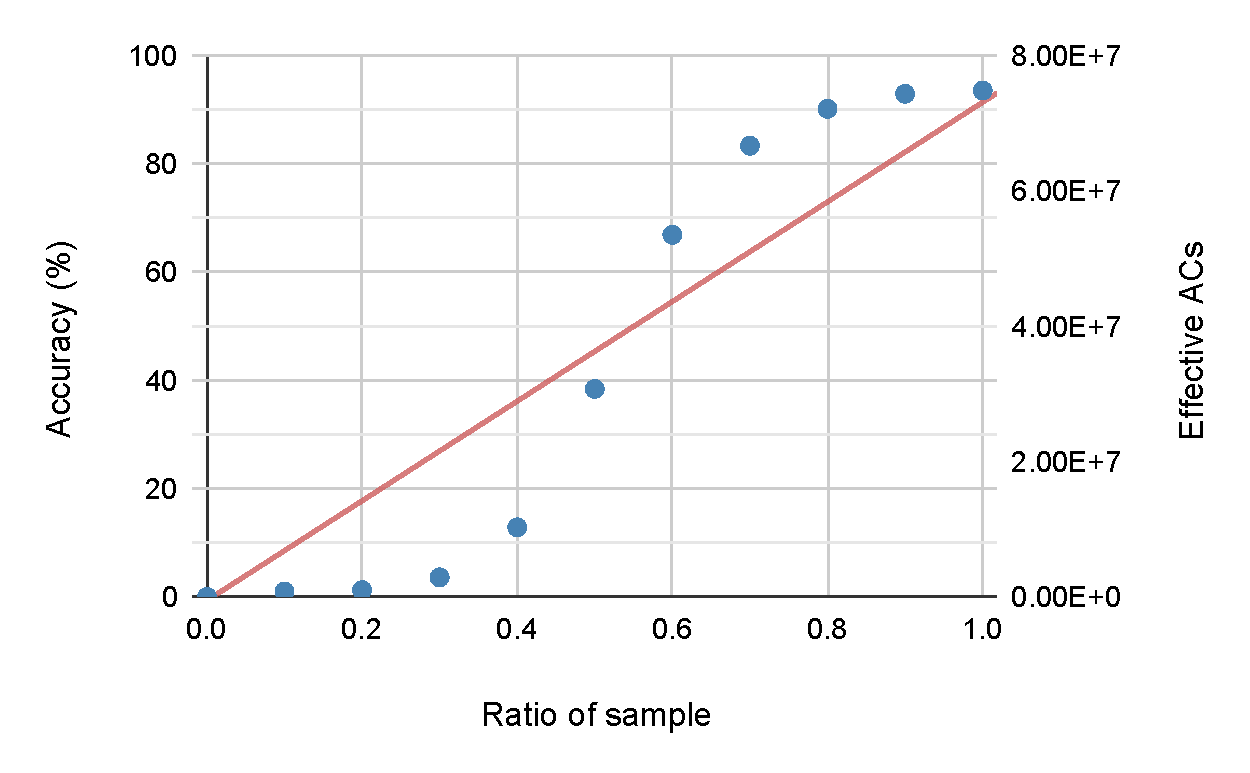
\includegraphics[width=.70\textwidth]{figures/snn_acc_compute_time.pdf}
    %             \caption{Test accuracy (blue) and aggregated effective ACs (red) of SNN on base classes using only the first portions of the keyword sample.}
    %         \label{fig:snn_acc_time}
    %     \end{figure}

% a base session with fixed classes, each with abundant training data, is used to train an initial model. Then, successive incremental training sessions introduce new classes in a few-shot learning scenario. In each session, only the current session classes are available to the model for training. After each incremental training session, the model is evaluated on all previously seen classes, including the base classes. Therefore, the model has to learn new classes while retaining knowledge about the previously learned ones. 

    % The keyword FSCIL task first uses a base dataset consisting of 100 base classes with abundant training data to pre-train models before proceeding with incremental learning on 100 extra classes. 
    After pre-training using standard batched training, the ANN and SNN baseline networks reach high accuracies on the base classes of 97.09\% and 93.48\%, respectively.
    % \red{The SNN solution, including the pre-processing, processes one input timestep at a time with a frequency of 200~Hz, compared to the ANN which requires a full one second sample to pass through the model. While the number of effective operations per-sample is lower for the ANN baseline, the SNN distributes computation temporally over 200 timesteps, thus its effective operations per model execution is one order of magnitude lower ($3.65 \times 10^5$).}
    As reported by the model execution rate metric, the SNN baseline computes each sample over 200 passes, using an order of magnitude fewer effective AC synaptic operations compared to the ANN baseline's effective MACs per model execution.
    Considering both the model execution rate and synaptic operation metrics, the number of aggregated ACs over the length of the sample ($200 * 3.65 \times 10^5 = 7.30 \times 10^7$) exceeds the Dense and effective MAC operations necessary for the ANN baseline, which spatially flattens the sample and processes it in one model execution.
    However, outside of the static-length keyword classification scenario, the low-cost per-execution temporal processing of SNNs can enable efficient, always-on, high-frequency prediction capabilities in deployed continuous audio recognition scenarios. 

    % Furthermore, the temporal processing of the SNN has capabilities to produce predictions before the sample is completed. 
    % Figure~\ref{fig:snn_acc_time} demonstrates that the SNN reaches 90\% accuracy using the first 80\% of the sample. Moreover, the number of aggregated effective ACs grows as a linear function of the sample ratio, demonstrating a compute reduction corresponding to the early prediction. Further research in online neuromorphic methods for fast time-to-prediction and compute-accuracy trade-offs\cite{jeffares2022spikeinspired} is enabled by the benchmark data features (see Methods section).
    

    \begin{figure}[ht]
                \centering
                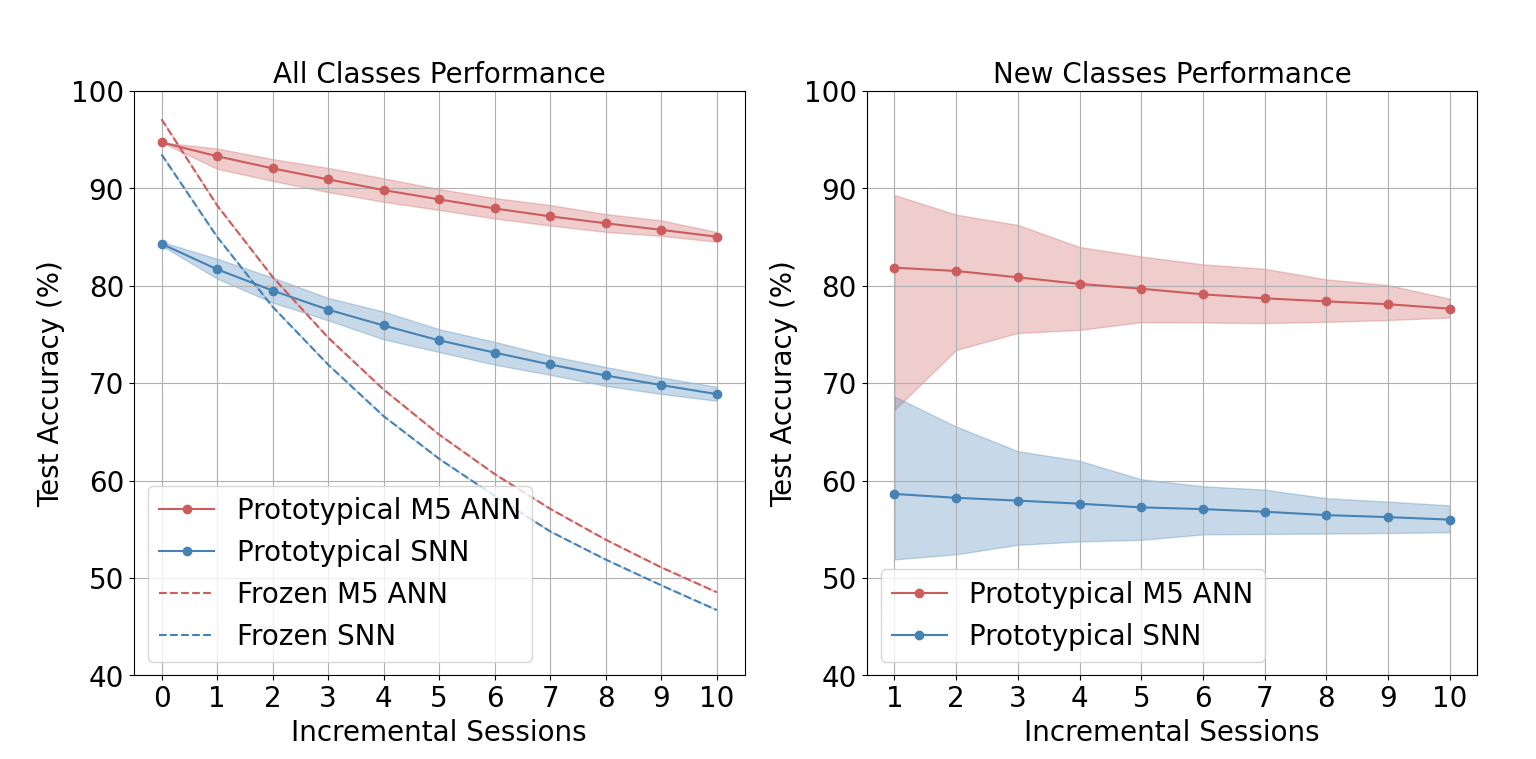
\includegraphics[width=\textwidth]{figures/FSCIL_proto.png}
                \caption{Test accuracy per session on the keyword FSCIL task for prototypical and frozen baselines, with the accuracy on both base classes and incrementally-learned classes (left), and accuracy on all incrementally-learned classes only (right). Incremental session 0 refers to the accuracy on base classes after pre-training only. Shaded area represents 5$^{th}$ and 95$^{th}$ percentile on 100 runs. Frozen baselines with no adaptation do not learn incremental classes and thus have a fixed 0\% accuracy for New Classes Performance. }
            \label{fig:mswc_acc_per_session}
        \end{figure}


    % For the incremental learning portion of the task, 10 successive sessions, each representing a new language, are presented to the model. Each session contains 10 new classes with 5 samples each (10-way 5-shot learning). This set-up 

% NEW VERSION WITH PROTOTYPES METHOD:

    % The 10-way, 5-shot class-incremental learning per incremental session poses the challenge of learning new classes while avoiding catastrophic forgetting, especially with the limited number of samples for new classes. We therefore present two reference solutions for both the ANN and SNN baselines: a \textbf{frozen} baseline with no weight updates in the incremental learning phase and a \textbf{prototypical} baseline that employs class prototypes~\cite{snell2017prototypical} for incremental learning. 
    % The frozen ANN and SNN have 0\% accuracy on incremental classes, and serve as reference for models which have no learning, but also no catastrophic forgetting of prior classes. 

    % In prototypical networks~\cite{snell2017prototypical}, all classes are associated with a \textit{prototype}, which is the average feature embedding, produced by the network before the readout classifier layer, over all training samples for each class. During inference, input samples are classified as the class corresponding to the prototype with the lowest squared Euclidean distance to the sample's embedding. Since computing this distance is equivalent to an affine operation on the feature embeddings~\cite{snell2017prototypical}, the prototypical network classifier can be expressed as a standard linear readout layer defined with respect to the prototype of each class. Thus, the final model consists of a prototype classifier output layer following the feature extracting hidden layers.

    % Although the original work on prototypical networks suggests a specific approach to train the feature extractor network~\cite{snell2017prototypical}, we employ standard pre-training with end-to-end backpropagation to enable high base class accuracy. After pre-training, the readout classifier layer is dropped, and the base classes prototypes and prototype layer are computed a-posteriori based on features from the hidden layers of the pre-trained network. This allows for common readout classification for base and incremental classes, however, it comes with an accuracy loss for base classes as the feature extraction in hidden layers is not trained with the classifier. 

    % The prototypical network approach is simple and computationally efficient, as no hyperparameters are used and parameters are not optimized, but instead calculated directly. 
    % Also, the prototypical evaluation method does not affect model complexity, as the prototypical classifier directly substitutes the default readout layer. Thus, the complexity results in Table~\ref{tab:FSCIL_results} empirically apply to both the frozen and prototypical models.

    % JY: compressed details from prior 4 paragraphs into this single paragraph, also compressed the following paragraphs
    We present two approaches for the incremental stage for both the ANN and SNN baselines. The \textit{frozen} models are locked after pre-training on base classes and have 0\% accuracy on all new incremental classes, providing a reference for models with no learning or catastrophic forgetting of prior classes. The \textit{prototypical} models employ a prototypical network~\cite{snell2017prototypical} for incremental learning, which is a feature-based clustering approach that can be implemented with a simple linear readout layer on top of the pre-trained network backbone. Prototypical weights and biases of prior and incremental classes are directly defined based on the average features of the corresponding class and directly substitute pre-trained readout layer parameters.  The complexity results in Table~\ref{tab:FSCIL_results} thus empirically apply to both the frozen and prototypical models.
    
    The test accuracy for the baseline models over all sessions, as well as the test accuracy on only the new incrementally-learned classes, are shown in Figure~\ref{fig:mswc_acc_per_session}.
    Using prototypical networks, the ANN model reaches 89.27\% accuracy on average over all sessions, demonstrating significant greater performance of 21.41 accuracy points with respect to the frozen model. The accuracy on new classes, averaged over all incremental sessions, is 79.61\%.
    The SNN prototypical baseline, on the other hand, reaches 75.27\% accuracy on average over all sessions, surpassing the frozen SNN performance by 9.97 accuracy points, with an average accuracy on new classes over all sessions of 57.23\%. 

    The accuracy loss over the incremental sessions is similar between the ANN and SNN prototypical baselines. However, the lower overall accuracy of the SNN is largely due to the conversion from the original backpropagation-trained readout classifier, which is used in the frozen baseline, to the prototype readout classifier. 
    On the base classes (session 0 in Figure~\ref{fig:mswc_acc_per_session}), the ANN sees a drop of 2.37\% between the frozen and prototypical baselines, while the SNN has a larger drop of 9.17\%. 
    The larger drop indicates that our particular SNN baseline has a less general feature extraction than the ANN. This may be due to the challenges of backpropagation through time for online temporal inference to learn to extract long-term temporal keyword features with the chosen spiking recurrent model. Additionally, the Speech2Spikes~\cite{stewart23speech2spikes} pre-processing algorithm converting audio to spikes may also cause information loss. Overall, the keyword FSCIL benchmark presents opportunities for further research in learning methods, preprocessing, and model architectures for continual learning of temporal data. 

    % A significant part of the gap in performance between the SNN and ANN prototypical baselines is due to the conversion from backpropagation-trained readout layer to prototype layer after pre-training, as the further accuracy drop over sessions is quite similar. Although the ANN also sees a drop of 2.37\% between the frozen and prototypical baselines at session 0, the impact on the SNN is notably bigger with a drop of 9.17\% due to the conversion. This can be explained by a less general feature extraction obtained with the SNN. The first hypothesis for that is that the online nature of the SNN, along with backpropagation through time, despite its computational advantage is making it harder for the network to extract long-term temporal features for the selected keywords. Additionally the pre-processing algorithm used to convert Spectrograms to spikes can create a loss of information as it has not been fine-tuned for this task. We want present this remaining gap between keyword spotting SNN and CNN models as an incentive for the community to keep researching this challenge in the direction of more refined pre-processings for SNNs and better architectures to extract robust temporal features.


    % Altogether, we nonetheless showed the ability of both ANN and SNN networks to demonstrate some class-incremental learning capacities with the prototypical networks method on this new keyword classification FSCIL task. This should serve as a simple reference to explore a challenge that is pushing the required learning and embedding capacities of neural networks to their fullest in a temporal domain setup.


% WEIGHT CONSOLIDATION (OLD METHOD) VERSION BELOW

    
    % The 10-way, 5-shot class-incremental learning per incremental session poses the challenge of learning new classes while avoiding catastrophic forgetting, especially with the limited number of samples for new classes. We therefore present two reference solutions for both the ANN and SNN baselines: a \textbf{frozen} baseline with no weight updates in the incremental learning phase and a \textbf{consolidated} baseline that employs a weight consolidation method~\cite{pellegrini20latent} for incremental learning. 
    % The frozen ANN and SNN have 0\% accuracy on incremental classes, and serve as reference for models which have no learning, but also no catastrophic forgetting of prior classes. The weight consolidation method for the consolidated baselines incrementally learn new classes by training only weights corresponding to newly learned classes in the output layer, centering weights around zero based on the average of newly trained weights. 
    % Notably, the weight consolidation method does not affect model complexity, thus the results in Table~\ref{tab:FSCIL_results} empirically apply to the frozen and consolidated models.
    
    % The \textbf{frozen} baselines keep the same parameters obtained in pre-training throughout all the incremental sessions. During pre-training, the 200 output neurons for the whole 200 final classes are present. Thus the \textbf{frozen} baselines present a 0 accuracy on all new classes as output weights to . They are nonetheless a relevant reference as 
    
    % the ANN baseline is trained with weight consolidation~\cite{pellegrini20latent} to learn the new classes. During each session of the FSCIL task, only the weights corresponding to the newly learned classes in the output layer of the model are trained using the few-shot training samples. Moreover, after all training sessions, including the pre-training, these weights are centered around zero based on the average on the newly trained weights. The test accuracy over sessions, as well as accuracy on only the incrementally-learned classes, is shown in Figure~\ref{fig:mswc_acc_per_session}.

    
    % The test accuracy for the baselines over all sessions, as well as the test accuracy on only the incrementally-learned classes, can be found in Figure~\ref{fig:mswc_acc_per_session}. 
    % Using weight consolidation, the ANN model reaches 85.70\% accuracy on average over all sessions, demonstrating significant relative improvement of 25.70\% with respect to the frozen model. This demonstrates the ability of the ANN solution to learn new classes from few-shot examples while limiting forgetting of previous classes. The accuracy on incremental classes, on average, is 64.48\%.

    % \red{For the SNN model, the same weight consolidation method used for the ANN did not provide an improvement on the default baseline with no incremental training, as the network either could not manage to learn new classes at all or new class predictions overshadowed the prediction of old classes and caused catastrophic forgetting. We therefore only provide the non-learning FSCIL baseline for the SNN model at this point, and motivate future research in adaptive few-shot, incremental learning in SNNs.}

    % The SNN baseline, on the other hand, reaches 66.23\% accuracy on average over all sessions, improving the frozen SNN performance by 1.43\% with an average accuracy on incremental classes of 3.87\%. \note{See note in Figure 4, exploring a better SNN baseline.} The observed limitation of weight consolidation with the SNN is a high sensitivity to the learning rate employed in incremental sessions. Low learning rates hinder the ability to learn new classes while greater rates cause catastrophic forgetting as the newly learned classes overshadow prior ones. 
    % The SNN baseline motivates further research into model architectures and learning rules for developing solutions to the FSCIL problem.
    % Contrary to the ANN solution, a sweep spot of learning rate with this weight consolidation could not be found. We make the hypothesis that this is due to the more sensitive nature of spiking neurons and of backpropagation through time, and incite the community to face this challenge to provide a more efficient solution to the FSCIL problem.

    

    % JY: we don't really have an SNN training method, so no need to mention training complexity?
    % We further note that the NeuroBench benchmarks do not yet specify metrics for model training complexity - all complexity metrics refer to model inference only. Future NeuroBench iterations will look towards training metrics, including potential solution-specific metrics for online weight adaptation, which can be measured during the few-shot training of the FSCIL task.

    
    \subsubsection*{Event Camera Object Detection}

    % \begin{table}[h]
% \centerline{
% \renewcommand{\arraystretch}{1.2}
% \begin{tabular}{|c|c|c|c|c|c|ccc|}
% \hline
% \multirow{2}{*}{Baseline} &
%   \multirow{2}{*}{COCO mAP} &
%   \multirow{2}{*}{\begin{tabular}[c]{@{}c@{}}Footprint\\ (bytes)\end{tabular}} &
%   \multirow{2}{*}{\begin{tabular}[c]{@{}c@{}}Frequency\\ (Hz)\end{tabular}} &
%   \multirow{2}{*}{\begin{tabular}[c]{@{}c@{}}Connection\\ Sparsity\end{tabular}} &
%   \multirow{2}{*}{\begin{tabular}[c]{@{}c@{}}Activation\\ Sparsity\end{tabular}} &
%   \multicolumn{3}{c|}{SynOps} \\ \cline{7-9} 
%         &       &          &    &     &       & \multicolumn{1}{c|}{Dense}    & \multicolumn{1}{c|}{Eff\_MACs} & Eff\_ACs \\ \hline
% RED ANN & 0.429 & $9.13 \times 10^7$ & 20 & 0.0 & 0.634 & \multicolumn{1}{c|}{$2.84 \times 10^{11}$} & \multicolumn{1}{c|}{$2.48 \times 10^{11}$}  & 0 \\ \hline
% Hybrid  & 0.271 & $1.21 \times 10^7$ & 20 & 0.0 & 0.613 & \multicolumn{1}{c|}{$9.85 \times 10^{10}$} & \multicolumn{1}{c|}{$3.76\times 10^{10}$}  & $5.60\times10^8$ \\ \hline
% \end{tabular}
% }
% \caption{Baseline results for the event camera object detection task.}
%     \label{tab:ObjDet_resuls}
% \end{table}

\begin{table}[ht]
\centerline{
\renewcommand{\arraystretch}{1.3}
\begin{tabular}{c|cccccccc} \thickhline
\multirow{2}{*}{Baseline} &
  \multirow{2}{*}{\begin{tabular}[c]{@{}c@{}}mAP\end{tabular}} &
  \multirow{2}{*}{\begin{tabular}[c]{@{}c@{}}Footprint\\ (bytes)\end{tabular}} &
  \multirow{2}{*}{\begin{tabular}[c]{@{}c@{}}Model Exec.\\ Rate (Hz)\end{tabular}} &
  \multirow{2}{*}{\begin{tabular}[c]{@{}c@{}}Connection\\ Sparsity\end{tabular}} &
  \multirow{2}{*}{\begin{tabular}[c]{@{}c@{}}Activation\\ Sparsity\end{tabular}} &
  \multicolumn{3}{c}{SynOps (per model exec.)} \\ \cline{7-9} 
        &       &          &    &     &       & \multicolumn{1}{c}{Dense}    & \multicolumn{1}{c}{Eff\_MACs} & Eff\_ACs \\ \hline
RED ANN & 0.429 & $9.13 \times 10^7$ & 20 & 0.0 & 0.634 & \multicolumn{1}{c}{$2.84 \times 10^{11}$} & \multicolumn{1}{c}{$2.48 \times 10^{11}$}  & 0 \\
Hybrid  & 0.271 & $1.21 \times 10^7$ & 20 & 0.0 & 0.613 & \multicolumn{1}{c}{$9.85 \times 10^{10}$} & \multicolumn{1}{c}{$3.76\times 10^{10}$}  & $5.60\times10^8$ \\ \thickhline
\end{tabular}
}
\caption{Baseline results for the event camera object detection task.}
    \label{tab:ObjDet_resuls}
\end{table}

    The event camera object detection task reports a prior baseline, the RED ANN, and a novel conversion of the architecture to a hybrid ANN-SNN model:
    
    \begin{itemize}
        \item \textbf{RED ANN} -- The RED architecture \cite{Perot2020} consists of blocks of feed-forward squeeze-and-excite~\cite{hu18squeeze} convolutional layers followed by blocks of recurrent convolution-LSTM (ConvLSTM~\cite{shi15convlstm}) layers.
        % The feed-forward convolutional layer is the squeeze-and-excitation layer for better performance. The recurrent convolutional layer is the ConvLSTM layer for effective temporal learning. 
        A single-shot detection (SSD~\cite{Liu_2016}) head is used to predict the location and class of the bounding box based on multi-scale outputs from the recurrent layers. 
        %The RED architecture has activation sparsity in the feed-forward convolutional layers. However, due to the activation function used, the ConvLSTM layers output dense activations. 
        Raw event data is binned into 50 ms and pre-processed into time surfaces. 
        %The model is trained using the SSD loss function consisting of a regression term for box coordinates and a classification term for the class. The selection of the SSD loss terms is the same as in the RED paper.
        \item \textbf{Hybrid} -- The hybrid ANN-SNN architecture adopts feedforward LIF spiking neural layers to replace the ConvLSTM layers in RED, and shares the same feed-forward convolutional blocks as the RED. It uses the same input encoding method and SSD head as the RED model. 
        % The model shares the same input encoding method, object detection head, and training loss functions as the RED model.
    \end{itemize}

    Results for the two networks can be found in Table \ref{tab:ObjDet_resuls}. The RED ANN represents the current state-of-the-art correctness on the benchmark, at 0.429 mAP. The Hybrid network is a smaller network, reflected by the footprint and synaptic operations metrics measuring an order of magnitude smaller than for the RED ANN. The smaller size comes at the expense of lower correctness of 0.271 mAP.

    For the RED ANN, the activation sparsity metric (0.634) represents zero activations by the ReLU function for each neuron. From this, one may expect that the number of effective operations (operations with a nonzero activation and nonzero weight) would be around 35\% of dense operations, however the actual ratio is 87\%. This is due to the presence of normalization layers applied to activations before synaptic weight multiplication. Furthermore, neurons with lower activation frequency in the network tend to have a smaller fanout than neurons with high activation frequency. Thus, while activation sparsity alone can provide a proxy for the cost of the network, architectural characteristics may impede actual computation reduction, and the synaptic operations must be considered in tandem.

    The Hybrid network demonstrates a significant reduction in total effective operations against dense operations, outlining significant gains if deployed on specialized sparsity-aware hardware. However, for the particular network, the number of effective ACs, generated by the spiking neuron components, is two orders of magnitude smaller than the number of effective MACs within the ANN components. Such a hybrid network may not warrant specialized accumulation units, and the baseline motivates further research in hybrid networks with a larger proportion of spiking neuron activity compared to artificial neuron activity.

    % Lastly, the connection sparsity metrics for both models is zero, indicating opportunities in weight pruning and sparse recurrent layers.

    \subsubsection*{NHP Motor Prediction}
\input{tables/primate_reaching_baselines}

    Small fully-connected, feedforward networks were developed for the NHP motor prediction baselines:
    
    \begin{itemize}
        \item \textbf{ANN} -- In the ANN baseline, the cortical activity from the 50 most recent data samples is buffered to be used as network input. The network has two hidden layers and $2$ final outputs predicting $X$ and $Y$ velocities, with a fully-connected topology of $N_{ch}$-32-48-2, where $N_{ch}$ refers to the channels of cortical data (96 for NHP Indy, and 192 for NHP Loco). Batch normalization is applied after each hidden layer.
        
        \item \textbf{SNN} -- The SNN uses the data samples directly as input to the network, without buffering. It has a hidden layer of 50 LIF neurons, for a fully connected topology of $N_{ch}$-50-2 LIF neurons. The output neurons do not have a reset mechanism, and the membrane potential is directly read to produce the output velocities. 
        
        % \TODO{Layernorm SNN with three layers vs Paul SNN with only two layers} The SNNs, similar to ANNs used a temporal window of $T_{BW}=200$ ms for the prediction. Similar to ANN$\_$V2, it splits this window into $n_p=7$ subsets, each of which corresponded to a timestep of the SNN. \red{The firing rates in each subset were binarized and fed as input to the SNN} to eliminate multiplications. Unlike the ANN$\_$V2, the input dimension remained equal to $N_{ch}$, reducing memory. However, computations were increased since all the layers had to be run for $n_p$ timesteps. For each new prediction, the SNN was reinitialized to operate over $n_p$ timesteps even though the current temporal window had overlap with the previous one. The SNN employed a fully connected topology $N_{ch}$-32-48-2. Since the task was regression, the neuron in the last layer did not have a reset mechanism, and the membrane voltage at the last time was considered as the output. Each membrane voltage was scaled by a learnt parameter to match the range of $X$ and $Y$ velocities.
    \end{itemize}

Table \ref{tab:primate_results} shows the results for the ANN and SNN baselines, averaged between sessions from each NHP (Indy and Loco). The ANN and SNN are similar in footprint size and number of dense operations per model forward pass, and also reach comparable prediction quality based on $R^2$ score. Each model is small in footprint and operation count, demonstrating that this task can be solved by shallow edge networks, validating prior studies~\cite{willsey22realtime}.

Between the baselines, the SNN realizes similar correctness at significantly reduced complexity compared to the ANN. Extremely high activation sparsity in the SNN (0.998) directly translates to low effective accumulate operations, demonstrating the adequacy of stateful, binary-activation neuron models for sparse regression tasks. Meanwhile, similarly to the RED ANN in the event camera object detection task, activation sparsity in the ANN baseline does not translate to effective operation efficiency, as batch normalization is applied to activations before multiplication with synaptic weights.

\begin{figure} [ht]
\centering
\begin{subfigure}{.5\textwidth}
  \centering
  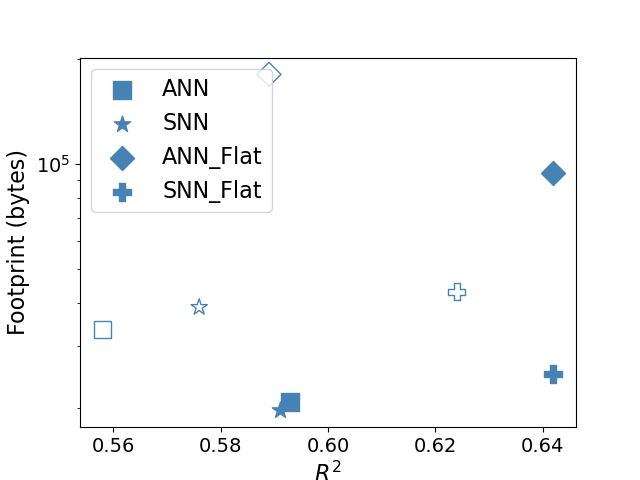
\includegraphics[width=1\linewidth]{figures/Memory_vs_Accuracy.png}
%  \caption{A subfigure}
  \label{fig:sub1}
\end{subfigure}%
\begin{subfigure}{0.5\textwidth}
  \centering
  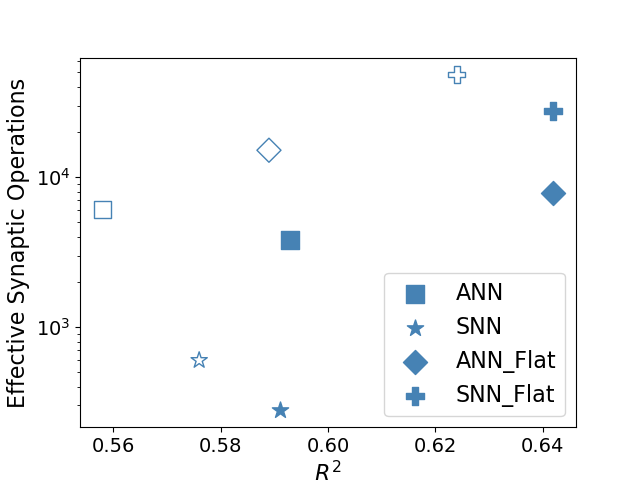
\includegraphics[width=1\linewidth]{figures/Computes_vs_Accuracy.png}
%\caption{A subfigure}
  \label{fig:sub2}
\end{subfigure}
\caption{Footprint and effective synaptic operations vs $R^2$, for four task baselines. Each model has two points: the solid marker represents NHP Indy, and the hollow marker represents NHP Loco.}
\label{fig:motor_result}
\end{figure}

We conduct further exploration for increasing task accuracies with more complex ANN and SNN models: ANN\_Flat and SNN\_Flat. For these networks, 50 data samples of buffered input are split into $n_p=7$ accumulated bins. For ANN\_Flat, the 7 bins are spatially flattened as input to the network, so its topology is ($7\times N_{ch}$)-32-48-2. 
SNN\_Flat uses the $N_{ch}$-32-48-2 topology, and the 7 bins are temporally flattened as input, presented to the network as separate input timesteps. Each prediction still uses the membrane potential of the output neurons after input timesteps, and the network is reset for each prediction. Layer normalization is also applied on the SNN\_Flat inputs.

Figure \ref{fig:motor_result} shows plots of complexity and predictive quality of all four baseline networks. Both flattened networks demonstrate significantly greater $R^2$ performance than the other two networks. However, the larger input dimension of the ANN\_Flat network is reflected in its greater footprint, and the increased model timesteps and layer normalization sharply increase the effective operations of SNN\_Flat by two orders of magnitude compared to the simpler SNN. Thus, while input flattening and normalization increase the quality of model predictions for ANNs and SNNs, each comes with a significant complexity trade-off. 
% Further research is motivated in computationally efficient model performance enhancement, such as weight plasticity or neuron models, that may be directly supported by neuromorphic hardware.



\subsubsection*{Chaotic Function Prediction}
% TODO: need to figure out how to cite and position in terms of existing benchmarking with MG: https://www.sciencedirect.com/science/article/pii/S2666827022000275
% \cite{shahi2022prediction}
% \begin{table}[ht]
% \centerline{
% \renewcommand{\arraystretch}{1.2}
% \begin{tabular}{|c|c|c|c|c|c|ccc|}
% \hline
% \multirow{2}{*}{Baseline} &
%   \multirow{2}{*}{sMAPE} &
%   \multirow{2}{*}{\begin{tabular}[c]{@{}c@{}}Footprint\\ (bytes)\end{tabular}} &
%   \multirow{2}{*}{\begin{tabular}[c]{@{}c@{}}Frequency\\ (Hz)\end{tabular}} &
%   \multirow{2}{*}{\begin{tabular}[c]{@{}c@{}}Connection\\ Sparsity\end{tabular}} &
%   \multirow{2}{*}{\begin{tabular}[c]{@{}c@{}}Activation\\ Sparsity\end{tabular}} &
%   \multicolumn{3}{c|}{SynOps} \\ \cline{7-9} 
%         &       &          &    &     &       & \multicolumn{1}{c|}{Dense}    & \multicolumn{1}{c|}{Eff\_MACs} & Eff\_ACs \\ \hline
% ESN & 14.79 & $2.81 \times 10^5$ & - & 0.876 & 0.0 & \multicolumn{1}{c|}{$3.52 \times 10^{4}$} & \multicolumn{1}{c|}{$4.37 \times 10^{3}$}  & 0 \\ \hline
% LSTM  & 13.37 & $4.90 \times 10^5$ & - & 0.0 & 0.530 & \multicolumn{1}{c|}{$6.03 \times 10^{4}$} & \multicolumn{1}{c|}{$6.03\times 10^{4}$}  & 0 \\ \hline
% \end{tabular}
% }
% \caption{Baseline results for the chaotic function prediction task. Frequency is not reported as the data is a synthetic time-series, with no real time correlation.}
%     \label{tab:MackeyGlass_resuls}
% \end{table}

\begin{table}[ht]
\centerline{
\renewcommand{\arraystretch}{1.3}
\begin{tabular}{c|cccccccc} \thickhline
\multirow{2}{*}{Baseline} &
  \multirow{2}{*}{\begin{tabular}[c]{@{}c@{}}sMAPE\end{tabular}} &
  \multirow{2}{*}{\begin{tabular}[c]{@{}c@{}}Footprint\\ (bytes)\end{tabular}} &
  \multirow{2}{*}{\begin{tabular}[c]{@{}c@{}}Model Exec.\\ Rate (Hz)\end{tabular}} &
  \multirow{2}{*}{\begin{tabular}[c]{@{}c@{}}Connection\\ Sparsity\end{tabular}} &
  \multirow{2}{*}{\begin{tabular}[c]{@{}c@{}}Activation\\ Sparsity\end{tabular}} &
  \multicolumn{3}{c}{SynOps (per model exec.)} \\ \cline{7-9} 
        &       &          &    &     &       & \multicolumn{1}{c}{Dense}    & \multicolumn{1}{c}{Eff\_MACs} & Eff\_ACs \\ \hline
ESN & 14.79 & $2.81 \times 10^5$ & - & 0.876 & 0.0 & \multicolumn{1}{c}{$3.52 \times 10^{4}$} & \multicolumn{1}{c}{$4.37 \times 10^{3}$}  & 0 \\ 
LSTM  & 13.37 & $4.90 \times 10^5$ & - & 0.0 & 0.530 & \multicolumn{1}{c}{$6.03 \times 10^{4}$} & \multicolumn{1}{c}{$6.03\times 10^{4}$}  & 0 \\ \thickhline
\end{tabular}
}
\caption{Baseline results for the chaotic function prediction task. Execution rate is not reported as the data is a synthetic time series, with no real-time correlation.}
    \label{tab:MackeyGlass_resuls}
\end{table}

The chaotic function prediction task has two recurrent ANN baselines, which feature distinct network architectures:

\begin{itemize}
        \item \textbf{Long short-term memory (LSTM)} -- LSTMs are a class of recurrent ANN architectures~\cite{Hochreiter1997}, utilizing multiple gates for selective retention or omission of past information. The LSTM baseline consists of a single LSTM with a hidden state of 100 neurons, followed by a feed-forward layer to produce single-dimension output predictions. 
        In addition, the LSTM baseline utilizes explicit memory by buffering 50 previous datapoints, spatially flattening them into 50 input channels.
        
        \item \textbf{Echo state network (ESN)} -- ESNs are randomized recurrent ANNs that belong to a class of algorithms known collectively as reservoir computing~\cite{ScardapaneRandomness2017}, featuring more biologically-inspired principles than LSTMs despite not being spiking networks. Standard ESNs have only one hidden layer (the reservoir), where synaptic connections projecting input data to the hidden layer and recurrent synaptic connections within the hidden layer are chosen randomly and stay fixed during the training. 
        % The only part of the network that is trained (referred to as the readout matrix) are the connections from the hidden and input layers to the output layer. 
        The model architecture for the ESN baseline has two neurons in the input layer, which projects the Mackey-Glass function input and additional constant bias input into a hidden layer of 186 neurons. Within the hidden layer, the probability of recurrent connections is set to 0.11. 
        % The training of the readout matrix was done using the standard teacher forcing procedure that, for the given time series, collected a matrix with activations of the input and hidden layers of the ESN and a vector with the corresponding ground truth values for the output layer.  This information was used to obtain the readout matrix with the regularized least squares estimator, Methods~\ref{sec:methods:algorithm:baselines}.
        
        
    
    \end{itemize}
The LSTM and ESN models were evaluated on a Mackey-Glass time series with $\tau=17$. The model is evaluated over 30 instantiations of the system; in each instance the start point is shifted forward by half of the Lyapunov time. The model is re-initialized and re-trained on each instance, and the results are averaged over all 30 instances. 

% JY: moved into methods
% The LSTM baseline shares characteristics with other baselines of a high effective-to-dense synaptic operation ratio, with a significant activation sparsity. Here, the internal sigmoid and $\tanh$ functions of the LSTM gates are not considered to be neuron activations, thus activations only account for the ReLU between the final LSTM cell and output layer. 

The ESN model is architecturally unique compared to the other ANN and SNN baselines. The connection sparsity metric ($0.876$) reflects the high number of zero-weight connections across its reservoir hidden layer. Due to this sparsity, hardware with support for sparse synaptic representation by ignoring zero weights would require less memory to represent the network, thus decreasing the deployed footprint of the model. The high connection sparsity of the ESN leads to significant reduction in synaptic operations - the ESN uses an order of magnitude fewer effective operations ($4.37\times10^3)$ than the LSTM ($6.03\times10^4$), while achieving comparable sMAPE. The activation sparsity of the ESN is 0 due to neurons using $\tanh(\cdot)$, rather than ReLU activations.



\begin{figure}[ht]
            \centering
            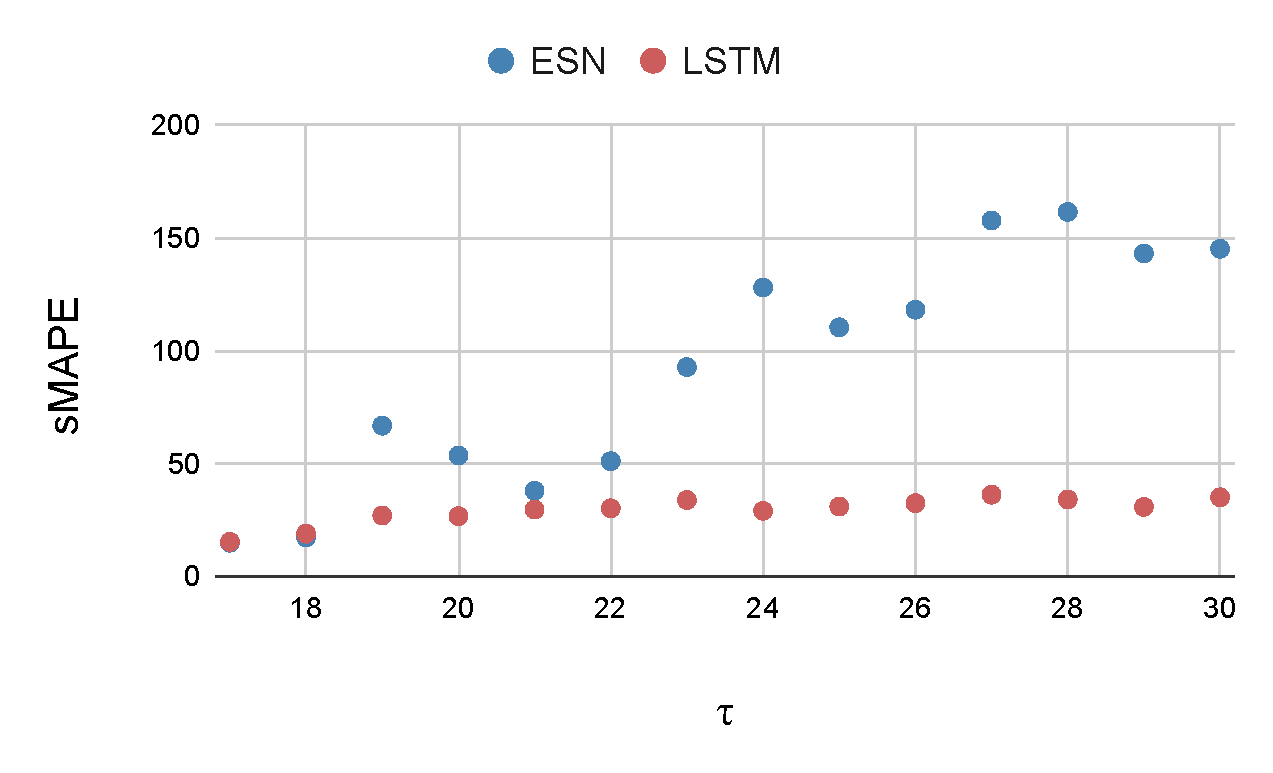
\includegraphics[width=.70\textwidth]{figures/mg_vary_tau.pdf}
            \caption{ESN and LSTM models evaluated on varying Mackey-Glass time series using a constant set of hyperparameters.}
        \label{fig:mackey_glass_function_performance}
    \end{figure}

Furthermore, we show the generalization and robustness capabilities of the particular ESN and LSTM models by applying them, with fixed hyperparameter sets, to other Mackey-Glass time series. Figure \ref{fig:mackey_glass_function_performance} shows the sMAPE score of the models over varied time series with the $\tau$ Mackey-Glass parameter varying between 17 and 30. The models were trained independently for each time series.
As the Mackey-Glass $\tau$ parameter characterizes the time-delay of the system, its increase roughly corresponds to prediction difficulty, shown by the increasing sMAPE trend through the plot. Notably, the LSTM maintains an error that is relatively lower than that of the ESN for all $\tau > 18$. However, the LSTM uses explicit memory via input buffering, so it is conjectured that the historical data allows for greater robustness to the varying time series characteristics. The ESN uses only one previous timestep, so its memory is only implicitly retained within its hidden layer. While the ESN tunes well to the $\tau$=17 case and demonstrates greatly reduced effective operations compared to the LSTM, the same set of hyperparameters does not generalize as well to other time series. Further research is motivated in explicit memory buffers versus implicit memory within the network state for trade-offs in single-series forecasting performance, complexity, and generalization capability.

\subsubsection*{Discussion and Opportunities for Further Research}
Baseline results for the four v1.0 algorithm track tasks compare the correctness and complexities of various solution types. Compared to ANNs, SNNs and ESNs demonstrate complexity advantages such as smaller footprints, high sparsity, and accumulate rather than multiply-and-accumulate operations. Especially on the motor prediction and chaotic function prediction regression tasks, the SNN and ESN baselines already achieve competitive correctness at lower complexity than the ANN and LSTM counterparts. Further research opportunities in model architectures, data pre-processing and buffering, and training paradigms to achieve greater performance is enabled by the standard framework and tooling provided by NeuroBench.
\section*{System Track Benchmark Framework}
% Target word count between 750 and 1000.

While the algorithm track aims to benchmark solutions in a system-independent manner via complexity analysis, the NeuroBench system track aims to evaluate deployed execution time, throughput, and efficiency of systems comprised of an algorithm deployed and tailored to a hardware platform. \secondrev{Previous benchmark studies have examined neuromorphic systems under various applications, including keyword spotting~\cite{blouw2019, bos2024micropowerspokenkeywordspotting}, audio and video processing~\cite{shrestha24efficient}, and combinatorial optimization~\cite{chen2024onoffneuromorphicisingmachines, pierro2024solvingquboloihi2}. While these studies have demonstrated neuromorphic system advantages, the benchmark tasks have been unaligned. In order for the hallmarks of neuromorphic hardware to be aptly judged against conventional systems and foster the expansion of neuromorphic solutions, transparent and objective comparisons must be made on standard tasks between sufficiently mature neuromorphic systems head-to-head, as well as against conventional systems.}

    \begin{figure}[ht]
            \centering
            
\includegraphics[width=.85\textwidth]{figures/system_types.png}
            \caption{Types of neuromorphic systems at various integration scales.}
        \label{fig:system_types}
    \end{figure}

A key challenge for benchmarking neuromorphic hardware is that systems are implemented and deployed at vastly different scales to serve diverse applications, from cloud services (e.g., multi-chip platforms like Loihi~\cite{Davies18loihi} and SpiNNaker~\cite{mayr2019spinnaker}) to embedded sensing intelligence (e.g., Speck~\cite{synsensespeck} and SNP~\cite{InnateraSNP, Levy2021}). This range is visualized in Figure~\ref{fig:system_types}. \secondrev{Existing benchmarks for conventional systems have individual focuses across high-performance~\cite{top500}, datacenter-level computing~\cite{Reddi2020}, and embedded processing~\cite{banbury2021mlperf}. 
Thus, rather than pursuing a one-size-fits-all suite of tasks, the goal of the NeuroBench system track is to develop benchmarks at various scales and use cases, under multiple application areas in which both conventional and neuromorphic platforms may compete. The selected v1.0 NeuroBench system track benchmarks represent key commercial application areas for existing systems, and they differ from the tasks in the algorithm track, which are more research-oriented. As benchmark results continue to identify properties of highly effective algorithms and systems, the two tracks will converge to the same selction of tasks that are seen as the most impactful for future progress in the field.}

\secondrev{In this section, we present the system track guidelines outlining metrics and tasks, representing collective design between multiple owners and vendors of neuromorphic hardware. Baseline benchmark results for neuromorphic and conventional systems are reported, and further official results will be collected and announced at a regular cadence, akin to the MLPerf suite~\cite{mlperf_policies}. As with all other facets of the NeuroBench framework, the system track guidelines will continue to be adapted and extended iteratively as benchmark results are produced and shared. Up-to-date information on the latest benchmarks and official results can be found on the NeuroBench website (\url{https://neurobench.ai/}).}

% As the system track benchmark tooling is currently under development, insight from the algorithm track's early results will be exploited towards a future release of the detailed harness documentation, benchmark procedure, and baselines for the system track by the end of 2024.

    \subsection*{System Track Metrics}
    \secondrev{In order to be representative of the properties of a deployed system, the system benchmarks, like the algorithm benchmarks, are assessed at the task level for the overall system, as opposed to operation- or kernel-level assessment of individual components. Task-level benchmarks enable straightforward comparison between systems of any type with regard to their abilities to solve problems, and the overall system-level measurement describes the realistic capability and efficiency of a whole solution.}

    \secondrev{Each individual system benchmark uses task-specific metrics aligned with \textit{correctness}, \textit{timing}, and \textit{efficiency} to measure the system under test (SUT). The following general considerations are applied to each category:}
    % % The following performance metrics describe what is considered a system-level evaluation. 
    % \sout{For ease of comparison and benchmark result analysis, key features of the NeuroBench system track are consistent with features from the widely-adopted machine learning  system benchmark MLPerf Inference~\cite{Reddi2020}.}

    % \TODO{Remove details about Task Scenarios, since it doesn't appear that the system benchmarks are consistent enough with the different scenarios. Make sure that the content serves the results report from Xylo.}

    % \paragraph{Task Scenarios.} Where applicable, the NeuroBench system track will utilize benchmark task scenarios from MLPerf. MLPerf describes task scenarios under which system benchmarks are presented to the system under test (SUT). For large-scale batched processing, MLPerf defines the \textbf{Offline} and \textbf{Server} scenarios, which are latency-unconstrained and latency-constrained, respectively, with performance measured in terms of prediction throughput. For batch-size-1 processing, MLPerf defines \textbf{Single-stream} scenarios, for which performance is measured in terms of prediction latency.

    % However, the MLPerf task scenarios all consider data as discrete samples, and therefore do not fit with some key neuromorphic system applications. The NeuroBench system track thus defines two additional task scenarios: \textbf{Real-time} and \textbf{Optimization}. \textit{Real-time} uses continuous data streams (e.g., from an event camera), which must be processed online by the SUT, in contrast with the \textit{Single-stream} scenario, where samples are sent only once the SUT has completed processing. Optimization applications use heuristic methods for otherwise intractable problems, and thus do not have notions of sample throughput or sample latency. The \textit{Optimization} scenario benchmarks will report latency for the SUT to reach multiple correctness thresholds, as many approaches find sucessively improved solutions over time.
    

    % For each task and scenario, the following metric categories are reported:
    \begin{itemize}
        \item \textbf{Correctness} -- \secondrev{In other system benchmarks, such as the closed category of the MLPerf Inference framework~\cite{Reddi2020}, the same trained model is used to benchmark all SUTs, and a correctness threshold is imposed to ensure optimizations such as lower precision do not disrupt task performance.}
        
        Due to the tight coupling between an algorithm and its system implementation in many existing neuromorphic hardware solutions, the particular model used to solve a NeuroBench system track benchmark task is unconstrained. Therefore, correctness must be measured to verify the validity of the solution. No correctness thresholds are imposed on submissions, but the benchmark leaderboard will impose tiers of solution correctness on submissions to evaluate accuracy-efficiency trade-offs of system approaches.
        
        \item \textbf{Timing} -- \secondrev{Depending on the task, timing performance can include measurements of sample throughput or execution time. Individually, the former entails an offline, batched inference benchmark, while the latter aligns with a streaming benchmark, in which one inference does not start until the previous one ends. Together, both throughput and execution time should be reported for tasks in which the SUT runs multiple inferences at any given time, each representing a request which must be responded to within a constrained window. The MLPerf Inference framework has defined widely-adopted general task scenarios corresponding to each of these categories (offline, single-stream, and server, respectively), and the NeuroBench system track will use these scenario guidelines where applicable to maintain consistency and build on conventional frameworks.}

        \secondrev{In addition, neuromorphic systems are also applied to tasks in which there is no notion of discrete sample throughput or execution, such as for heuristic approximations of intractable problems or operation over a continuous stream of data (e.g., from an event camera). Timing performance should be defined on a per-benchmark basis for such tasks, such as a time-to-solution latency or percentage of execution which exceeds a real-time threshold.}
        
        % Depending on the task scenario, the performance of the system is measured differently. The \textit{Offline} and \textit{Server} scenarios report throughput, while the \textit{Single-stream} scenario reports latency. The \textit{Real-time} scenario similarly reports latency, which for a large portion of execution (e.g., 90\%, defined per-benchmark) must not exceed a real-time threshold, or else the submission is not considered valid. The \textit{Optimization} scenario reports the time to solution at various solution quality thresholds, defined per-benchmark.
        
        \item \textbf{Efficiency} -- 
        Conventional system benchmarks such as TOP500~\cite{top500} for HPC and MLPerf Inference~\cite{Reddi2020} for deep learning do not require power measurement submission in the main benchmark, instead allowing for separate submissions to an adjacent power track (Green500~\cite{green500} and MLPerf Power~\cite{mlperfpower}, respectively). Not only has efficiency been usually considered as a second-order metric for conventional systems, it is also notoriously difficult to precisely measure. However, as energy efficiency is a key hallmark of biology and thus is a focus of neuromorphic research, power and energy consumption must be first-order metrics in the NeuroBench system track. \secondrev{Similarly to timing metrics, efficiency metrics should be tailored on a per-benchmark basis, i.e., a real-time always-on processing task may focus on average power, while offline batched systems focusing on high-throughput inference may focus on both peak power and energy per inference.}
        
        % The \textit{Server}, \textit{Offline}, and \textit{Real-time} scenarios report average power as their batched and online processing is continuous, the \textit{Single-stream} scenario reports the energy per-sample, and the \textit{Optimization} scenario reports total energy consumed at each solution quality threshold.
        
        % For tasks in the offline and server scenarios, average power is measured, while single-stream task scenarios intended for edge devices measure average energy consumption per sample. Further information about the power measurements is provided in the Methods section.
        
    \end{itemize}

    \secondrev{As neuromorphic systems currently explore a broad range of varied implementation approaches, board-level integration, and developmental stages of hardware, platform diversity poses difficult challenges for completely consistent hardware measurement methodologies (e.g., consistent power meters, chip interfaces, and data loading). Thus, to enable an initial step towards consistency in the system track while ensuring openness, we focus on the development of guidelines for transparent documentation, as they provide the foundation for shared methodology among highly diverse solutions. While there may be differences in how metrics are measured, salient details will be available to contextualize the results, allowing for holistic analysis, and leading the way for future consistency by enforcing transparency.}

    Benchmark submissions may perform separate runs to report performance and power in order to demonstrate system flexibility (e.g., a `performance-mode' run optimal for execution time and an `efficiency-mode' run optimal for energy), however in all runs, both metrics must be reported.

    Importantly for the NeuroBench system track, in measuring timing and efficiency, data pre- and post-processing must be taken into account. Neuromorphic methods will often consume and produce non-standard (e.g., event-based) data modalities, the processing of which may consume a significant amount of the overall execution time and may not be computed on the neuromorphic hardware itself. As many instances of neuromorphic hardware cannot be deployed without such associated processing, it is essential that measurements capture the cost of data processing, which stands in contrast with conventional system benchmarks whose measurements start from pre-processed data~\cite{mlperf_policies}.

    % \revision{Correctness and performance metrics are relatively straightforward to implement consistently across systems, and specific rules and measurement guidelines from MLPerf Inference~\cite{Reddi2020} will be used where applicable, with benchmark-specific modifications. However, due to the highly varied implementation approaches, board-level integration, and developmental stages of neuromorphic hardware, a first step towards 

    % \revision{Neuromorphic hardware may be implemented as a standalone system which covers the whole processing pipeline from raw data to prediction. However, the hardware may also be integrated as an accelerator unit which relies on a host CPU for pre-/post-processing. For standalone systems, performance and efficiency measurements must be monitored at the full-chip level. For accelerator systems, all processing from host integration must be included in the measurements, however the aggregated results should be broken into the host and neuromorphic components so that the full system can be characterized. Detailed hardware measurement guidelines are included in the Methods section.} \TODO{Check here}

    % \TODO{Integrate the following text:}

    % \revision{Where applicable, rules and measurement guidelines from MLPerf Inference~\cite{Reddi2020} will be used. Accuracy and performance (latency or throughput) can be measured in accordance with these rules and as noted further by the individual benchmarks.}

    % \revision{However, due to the highly varied implementation features, board integration, and developmental progress of neuromorphic hardware, an initial benchmark framework cannot expect fully consistent power measurement across all systems. Thus, power measurement is instead standardized under a common transparent documentation structure, such that while results may not be directly comparable, there is still the ability to holistically analyze results and move towards future consistency.}
    
    % \revision{The NeuroBench power specification highlights component-level granularity and inclusion of all pre-/post-processing hardware. 
    % Any on-board components which contribute to workload calculation should be included.} \TODO{List further notes about power spec or where it will be defined. Or maybe don't include further detail and instead move the prior paragraph up into the main text? It is an important idea.}

    \subsection*{System Track Benchmarks}
    \secondrev{Two benchmark specifications for the v1.0 system track are defined in this article, covering embedded to datacenter scales. Full benchmark details are available in the Methods section.}
    \begin{itemize}
        \item \textbf{Acoustic Scene Classification} -- The acoustic scene classification benchmark challenges systems to classify audio into predefined categories based on the environmental audio context. 
        % Utilising such an application as a vehicle for benchmarking is beneficial from varied perspectives. Real-world applicability of the use case can relatively easily be seen within, for example, hearables to adjust sound equalisation profile, to more appropriately target microphone noise cancellation or to support active noise cancellation. 
        Such capabilities are key for hearable devices, which can utilize them to automatically adjust sound equalisation profiles, appropriately target microphone denoising, and support active noise cancellation.
        The application further challenges systems to fulfill technical requirements, such as always-on and real-time operation, and time series processing.
        Acoustic scenes provide a rich repertoire of features that are necessary for prediction, thus this task is a complement to keyword classification, which mainly focuses on shorter-term features (e.g., phonemes) with a relatively smaller feature repertoire.
        % Furthermore, the chosen dataset and application would impart a requirement on the model and system to process and interpret a wide and rich repertoire of features in order to correctly produce a prediction. This task could complement that of keyword spotting which mainly focuses on shorter-term features (for example, phonemes) that are part of a relatively smaller repertoire.  

        % Leveraging the datasets from the DCASE~\cite{Heittola2020} challenge, we establish an acoustic scene classification benchmark that would evaluate the classification capabilities of both neuromorphic systems and conventional computing platforms. 
        
        The benchmark evaluates the classification capabilities of both neuromorphic systems and conventional computing platforms using \revision{datasets from the DCASE challenge~\cite{Heittola2020}.} 
        %(if permissible, subject to license).
        These datasets consist of a myriad of audio recordings from diverse environments, including airports, public parks, and buses, thus providing a comprehensive foundation for testing both application- and system-level performance. \secondrev{The NeuroBench subset of the DCASE dataset includes 41360/16240 train/test samples across four classes (airport, street traffic, bus, park).}
        % While the goal of an application-level task could be to also assess the generalisation performance, as stated as goal within the DCASE challenge itself, the system track would not necessarily enforce such stringent accuracy targets.

        % JY: attempted to fit this task into the Real-time task scenario, as it would be most coherent to provide specs for both the Real-time and Optimization new task scenarios.
        \secondrev{The task will be presented under the single-stream task scenario, providing one 1-second sample to the SUT at a time. Classification probability will be sampled to determine the correctness of the prediction. As the NeuroBench system track allows for unconstrained algorithmic implementation, pre-processing and inference metrics should be separately measured and reported together, which differs from prior system benchmarking that only measure inference~\cite{blouw2019, banbury2021mlperf}. 
        Timing results report on-device average execution time per sample.
        Since the platform diversity of edge-targeted systems poses inherent inconsistencies in efficiency measurement, power should be reported under idle and active contexts, following prior benchmark study methodology~\cite{blouw2019}. Idle power measures the system prepared for inference with the model loaded, and active power measures the system running pre-processing or inference. The difference between active and idle measurements offers dynamic power, which is used along with execution time to calculate dynamic energy-per-sample.}
        % The average power measured during inference is a key indicator of the efficiency and always-on capability of the SUT, and inference latency will be measured in terms of the prediction time relative to the onset of each new acoustic scene.
        
        % The metrics produced within this system track benchmark are: average power per inference, accuracy across a validation dataset, average inference latency. As in the case of the QUBO task and depending on the chosen solution, the impact of inference duration may be traded off to evaluate accuracy or energy scaling. In opposition to the QUBO task, the scale of the problem cannot be arbitrarily varied, therefore there exists the possibility that certain systems may be over or under-sized, and therefore power or accuracy may be scaled proportionally. The task would be profiled mainly in a single-stream fashion, wherein individual 1 second samples are used to report the above KPIs. The samples could also be stitched together to emulate a real-time scenario, however this may impose a restriction on the number and type of devices that can participate in the benchmark as storing many second samples may be outside of the ability of certain systems. 

        

        \item \textbf{QUBO} -- % Neuromorphic systems have repeatedly excelled in mathematic optimization heuristics. These tasks optimize a cost function by iterative updates of a large range of variables, operations that benefit from the tight compute-memory integration and massive parallelism of neuromorphic processors \cite{Aimone2022}. 
        As a non-ML task, NeuroBench incorporates quadratic unconstrained binary optimization (QUBO). QUBO is a particularly beneficial first optimization task for NeuroBench for two reasons. First, the binary variables are a natural fit for neuromorphic systems with purely binary spike communication. Second, real-world QUBO applications typically feature sparse cost matrices~\cite{koch2022} which benefit from the sparse synaptic connectivity and execution that neuromorphic systems are often optimized for \cite{Aimone2022}. The initial set of QUBO workloads in NeuroBench searches for the maximum independent (i.e. unconnected) set of nodes in graphs, a task that has wide applications across industry and academia, such as resource allocation in wireless networks, portfolio optimization, and task scheduling~\cite{wurtz2024industryapplicationsneutralatomquantum}.
        % Correctness of the task is the largest independent set found by the SUT, and it is compared in relation to the best result known for a particular dataset.
        
        NeuroBench provides a QUBO generator that can uniquely specify each workload by three specific parameters provided by the benchmark: the number of graph nodes, the density of graph connections, and a random seed. The generator provides a large dataset for reliable statistics and allows scaling from modest workloads for small-scale and prototype systems to large workloads for larger-scale systems. \secondrev{The graph sizes specified by the benchmark increase in a pseudo-geometric progression (10, 25, 50, 100, 250, ...), and submissions are encouraged to extend the problem size to the limits of the SUT. Graph density ranges from 1\% to 30\%, in order to show the relationship between the number of connections and SUT power. 5 random seeds for each setting should be tested.}
        % As an \textit{Optimization} scenario task, the time-to-solution latency aggregated energy consumption at various correctness thresholds is measured. In addition, the maximum supported workload size is reported.
        % The SUT is evaluated based on three metrics: The first success metric is the maximum supported workload size. The second and third metric is the time and energy required to obtain pre-defined levels of optimality, respectively. The solution optimality is measured by the size of the independent set of nodes found by the SUT.

        % The SUT is evaluated based on three metrics: The first success metric is the maximum supported workload size. The second and third metric is the timing and energy efficiency of the system, respectively. For optimization algorithms, these metrics can be measured in either of two ways: The first version of NeuroBench will measure the solution optimality and energy consumption reached during a pre-set runtime. The second version of NeuroBench will add a benchmarking routine that defines a target solution optimality and determines the time and energy required to achieve it, which will be released once reasonable target solution optimality have been determined using runs of conventional reference solvers. The solution optimality is measured by the cost of the QUBO cost function for the variable assignment obtained by the SUT.

        \secondrev{Optimization algorithms use heuristic methods to iteratively refine approximate solutions to intractable problems that cannot be completely solved. The QUBO benchmark thus measures solution optimality and energy consumption after fixed, pre-set runtimes, removing any timing measurement. Solution optimality is defined as BKS-Gap, a relative gap between the current SUT's solution compared against the best-known solution (BKS) to the same problem found using a high-powered solver with a long runtime.
        % Thus, the QUBO task is presented under two scenarios. The first is to measure solution optimality and energy consumption after fixed, pre-set runtimes, removing any timing meaesurement. The second is to define thresholds of solution optimality for given problems, and measure the latency and energy required for the SUT to reach each threshold. Solution optimality is defined as BKS-Gap\%, a relative gap between the current SUT's solution compared against the best-known solution (BKS) to the same problem found using a high-powered solver with a long runtime. Both scenarios are representative of optimization applications, so NeuroBench defines specifications for each. In this article, baselines for the former scenario are reported.
        }
        
        % \secondrev{In addition to timing and efficiency measurements under the two QUBO scenarios, when comparing neuromorphic systems head-to-head, each SUT should report the maximum supported workload size. While this may not be as important for von Neumann architecture systems with expandable working memory, neuromorphic systems often have co-located memory with processing, thus the metric highlights the scale of the SUT.}

        % JY: Commenting out these details for this paper
        % A community-wide benchmark must use protocols that support all hardware vendors. 
        % The first QUBO benchmark adopts QUBO problems where the Q-matrix can be represented by weights of at most 8-bit precision, aligned with the precision of synaptic weights in baseline neuromorphic systems. 
        % The Maximum Independent Set, for instance, requires both positive and negative weights but can be accommodated by eight bit precision. These values encode the presence or absence of an edge between two graph vertices. 
        % With increasing iterations, NeuroBench will also provide QUBO workloads that require greater weight precision to accompany and push the advancement of neuromorphic systems.
    
    \end{itemize}

% \subsection*{System Track Harness}
% \begin{figure}[ht]
%     \centering
%     \includesvg[width=.95\textwidth]{figures/alg_system_harness.svg}
%     \caption{\revision{An overview of the NeuroBench harness with support of the system track. The implementations of the system track components shown in blue are currently specific to the hardware backend, and common interfaces within the runtime allow that the harness can be modularly extended to various system backends.}}
%     \label{fig:alg_system_harness}
% \end{figure}

% \TODO{Considering again removing the system track harness figure, there are only shared data / task files and specifications in a repo. We can instead position the harness as a platform for which different systems can open-source their benchmarking scripts.}

% A diagram of the NeuroBench harness with extended support for the system track is shown in Figure~\ref{fig:alg_system_harness}. Blue boxes in the figure denote hardware-specific infrastructure components which will connect to the general top-level harness interfaces.

% \revision{Software toolchains such as Lava~\cite{lava}, Fugu~\cite{aimone2019composing}, NIR~\cite{NIR2023}, SPyNNaker~\cite{spynnaker}, Samna~\cite{samna}, among others, have been developed to interface with specific hardware platforms. Many of the stacks are built with general paradigms to support extension to any backend, and the community is actively moving towards developing standards for deployment tools.}

% \revision{In order to facilitate systematic hardware benchmarking in the present and further extensions in the future, the NeuroBench harness provides common interfaces within the runtime to allow modular execution for various backends. Initially, these components will be implemented using hardware-specific tools to optimize system benchmark performance. As standards mature, common tools such as model description frameworks and intermediate representations (IR) can be incorporated, reducing implementation complexity for benchmark users to test on many different platforms.}

% The side-by-side harness runtimes for the algorithm track and system track benchmarks provides users with a single tool for both types of analysis. As the algorithm and system tracks mature to support the same tasks, the harness will accelerate benchmarking by facilitating quick prototype complexity analysis followed by deployed performance measurement with minimal implementation overhead.

\subsection*{Baseline Results}

\secondrev{Baseline results for each of the two system track benchmarks are provided for a mature neuromorphic system against a conventional platform. Like for the algorithm track baseline results, the system track baselines are intended to snapshot the solution space and provide starting points for the task leaderboards. Further details on each baseline system are available in the Methods section, and in-depth system documentation for the Xylo ASC baseline and CPU/Loihi 2 QUBO baselines are provided by Ke et al.~\cite{ke2024neurobenchdcase2020acoustic} and Pierro et al.~\cite{pierro2024solvingquboloihi2}, respectively.}

\subsubsection*{Acoustic Scene Classification}


\secondrev{For the acoustic scene classification task, two baseline embedded systems are reported:
\begin{itemize}
    \item \textbf{CPU} -- The CPU baseline is an Arduino Nano 33 BLE, which uses an ARM Cortex M4 microcontroller for both pre-processing and inference. The digital audio sample is pre-processed using Mel-filterbank energies (MFE), and inference uses a conventional CNN. Execution time is measured using on-chip timers, and power is measured using total system power.
    \item \textbf{Xylo} -- The Synsense Xylo~\cite{synsensexylo} neuromorphic baseline uses a feed-forward SNN with multiple synaptic time constants~\cite{bos2024micropowerspokenkeywordspotting}. As the system is intended for continuous, real-time audio processing, the board uses an analog front end to pre-process analog audio signals directly from a microphone into spikes for the digital inference engine. To conform with a digital benchmark dataset, a simulator of the analog pre-processor generates spikes, which are routed to the inference module. Execution time and power are measured using on-board instruments.
\end{itemize}}

\begin{table}[ht]
\centerline{
\renewcommand{\arraystretch}{1.3}
% \begin{tabular}{@{}c|ccccccc@{}}
% \begin{tabular}{@{}c|cccccc@{}}
% \thickhline
% \multirow{2}{*}{Baseline} &
%   \multirow{2}{*}{Accuracy} &
%   \multirow{2}{*}{\begin{tabular}[c]{@{}c@{}}Latency\\ (ms)\end{tabular}} &
%   \multirow{2}{*}{\begin{tabular}[c]{@{}c@{}}Idle \\ Power (mW)\end{tabular}} &
%   \multirow{2}{*}{\begin{tabular}[c]{@{}c@{}}Active\\ Power (mW)\end{tabular}} &
%   \multirow{2}{*}{\begin{tabular}[c]{@{}c@{}}Dynamic \\ Power (mW)\end{tabular}} &
%   % \multirow{2}{*}{\begin{tabular}[c]{@{}c@{}}Active\\ Energy (mJ/inf)\end{tabular}} &
%   \multirow{2}{*}{\begin{tabular}[c]{@{}c@{}}Dynamic\\ Energy (mJ/inf)\end{tabular}} \\
%                       &                          &     &       &        &       &        &        \\ \hline
%           CPU         & \multirow{2}{*}{79.64\%} & 43  & 79.40 & 100.72 & 21.32 &  4.33  & 0.917   \\
%     (\textit{system-wise}) &                     & 45  & 79.40 & 100.15 & 20.75 &  4.51  & 0.934   \\ \hline
% Xylo & \multirow{2}{*}{76.00\%} & \textbf{N/A} & \textbf{N/A}   & 0.015  & \textbf{N/A}   & \textbf{N/A}    & \textbf{N/A}    \\
%  (\textit{component-wise})&                      & 40  & 0.298 & 0.503  & 0.205 & 0.0201 & 0.0082 \\ \thickhline
% \end{tabular}
%%%%%%%%%%%%%%%%%%% JY: The below block is the updated numbers / format
\begin{tabular}{@{}cc|cccccc@{}}
\toprule
\multicolumn{2}{c|}{\multirow{2}{*}{Baseline}}                        & \multirow{2}{*}{Accuracy} & \multirow{2}{*}{\begin{tabular}[c]{@{}c@{}}Execution\\ Time (ms)\end{tabular}} & \multirow{2}{*}{\begin{tabular}[c]{@{}c@{}}Idle \\ Power (mW)\end{tabular}} & \multirow{2}{*}{\begin{tabular}[c]{@{}c@{}}Active\\ Power (mW)\end{tabular}} & \multirow{2}{*}{\begin{tabular}[c]{@{}c@{}}Dynamic \\ Power (mW)\end{tabular}} & \multirow{2}{*}{\begin{tabular}[c]{@{}c@{}}Dynamic\\ Energy (mJ/inf)\end{tabular}} \\
\multicolumn{2}{c|}{}                                                 &                           &                                                                         &                                                                             &                                                                              &                                                                                &                                                                                    \\ \midrule
\multicolumn{1}{c|}{CPU}                       & \textit{pre-process} & \multirow{2}{*}{79.64\%}  & 43                                                                      & 79.40                                                                       & 100.72                                                                       & 21.32                                                                          & 0.917                                                                              \\
\multicolumn{1}{c|}{\textit{(system-wise)}}    & \textit{inference}   &                           & 45                                                                      & 79.40                                                                       & 100.15                                                                       & 20.75                                                                          & 0.934                                                                              \\ \midrule
\multicolumn{1}{c|}{Xylo}                      & \textit{pre-process*} & \multirow{2}{*}{79.90\%}  & -                                                                       & 0.00017*                                                             & 0.015*                                                                        & 0.015*                                                               & 0.015*                                                                                  \\
\multicolumn{1}{c|}{\textit{(component-wise)}} & \textit{inference}   &                           & 84                                                                      & 0.351                                                                       & 0.692                                                                        & 0.341                                                                          & 0.028                                                                             \\ \bottomrule
\end{tabular}
}
\caption{\secondrev{Baseline results for the acoustic scene classification task. Pre-processing of the Xylo (marked with an asterisk *) measures power of the analog pre-processor in real-time relative to the audio data, whereas other measurements are of digital components processing digital data on-hand. Idle Xylo pre-processing measures silence and active measures test data audio played to the device, and energy is measured over the sample duration of 1 second. CPU power is measured over the full Arduino system, as it does not have on-board power instrumentation, while Xylo power measures power consumed by the Xylo Audio 2 ASIC only. Dynamic power and energy provide proper comparison between the systems, and idle and active measurements are provided for transparency.}}
\label{tab:asc_results}
\end{table}



\secondrev{Table~\ref{tab:asc_results} lists baseline results for the neuromorphic Xylo system against an Arduino system. Compared to prior neuromorphic audio system benchmarking~\cite{blouw2019}, which takes a server-class CPU as a point of comparison, we adopt a fairer approach by focusing on low-power edge application and comparing against an Arduino embedded microprocessor. At comparable inference accuracy, Xylo exhibits $60.9\times$ less dynamic inference power and $33.4\times$ less dynamic inference energy consumption than the Arduino.
%Full details about the Xylo SNN, training, and measurement methodology are avaiable in Ke et al.~\cite{ke2024neurobenchdcase2020acoustic}
%Though this platform serves as a suitable comparison against the Xylo, the Arduino does not include any power instruments on-board or on-chip, and thus full system power must be measured externally. Meanwhile, the Xylo measures from on-board current instruments. The inconsistency is addressed by separating dynamic power as the difference between idle and active power measurements, though all are reported for transparency.
}

% \secondrev{The Edge Impulse platform~\cite{hymel2023edgeimpulsemlopsplatform} used to deploy the CPU baseline consists of commercially-developed tinyML optimizers and libraries for microcontroller devices such as the Arduino. At comparable inference accuracy, Xylo exhibits $60.9\times$ less dynamic inference power and $33.4\times$ less dynamic inference energy consumption than the Xylo. Full details about the Xylo SNN, training, and measurement methodology are avaiable in Ke et al.~\cite{ke2024neurobenchdcase2020acoustic}}

\subsubsection*{QUBO}
% \begin{table}[ht]
\centerline{
\renewcommand{\arraystretch}{1.5}
\begin{tabular}{c|cc}
\thickhline
\multirow{2}{*}{Baseline} &
  \multirow{2}{*}{\begin{tabular}[c]{@{}c@{}}Avg.\\ BKS-Gap \%\end{tabular}} &
  \multirow{2}{*}{\begin{tabular}[c]{@{}c@{}}Avg. Runtime \\ Power (W)\end{tabular}} \\
           &      &       \\ \hline
CPU - SA   & TODO & 87.78 \\ \hline
CPU - TABU & TODO & 97.56 \\ \hline
Loihi 2    & TODO & 2.62  \\ \thickhline
\end{tabular}
}
\caption{\secondrev{Baseline results for the QUBO task. Avg. BKS-Gap\% measures the average gap percentage between the solution found by the SUT and the best-known solution, averaged across fixed timeouts from $10^{-3}$ to $10^{2}$ seconds, graph sizes of $10^1$ to $10^3$, and graph density of 15\%. Average runtime power is measured over graph sizes of $10^1$ to $10^3$, and densities of 5\%, 15\%, and 30\%. Figures~\ref{fig:qubo_bksgap} and~\ref{fig:qubo_power} provide the breakdown of these results.} \TODO{Doesn't make sense to have a table since graph size changes things a log, and power increases as a function of graph size. Intel also prefer to keep the credit for their results, which means this benchmark will appear to be a copy.}}
\label{tab:qubo_results}
\end{table}
 
% \JY{TODO: The latest from Intel is that that they have lost the results for producing the figures, and would not prefer to spend the time to re-generate all of them. So all we have are the figures from their paper and a few numbers. Removed table.}

\begin{figure}[t]
    \centering
    \begin{subfigure}{0.48\textwidth}
        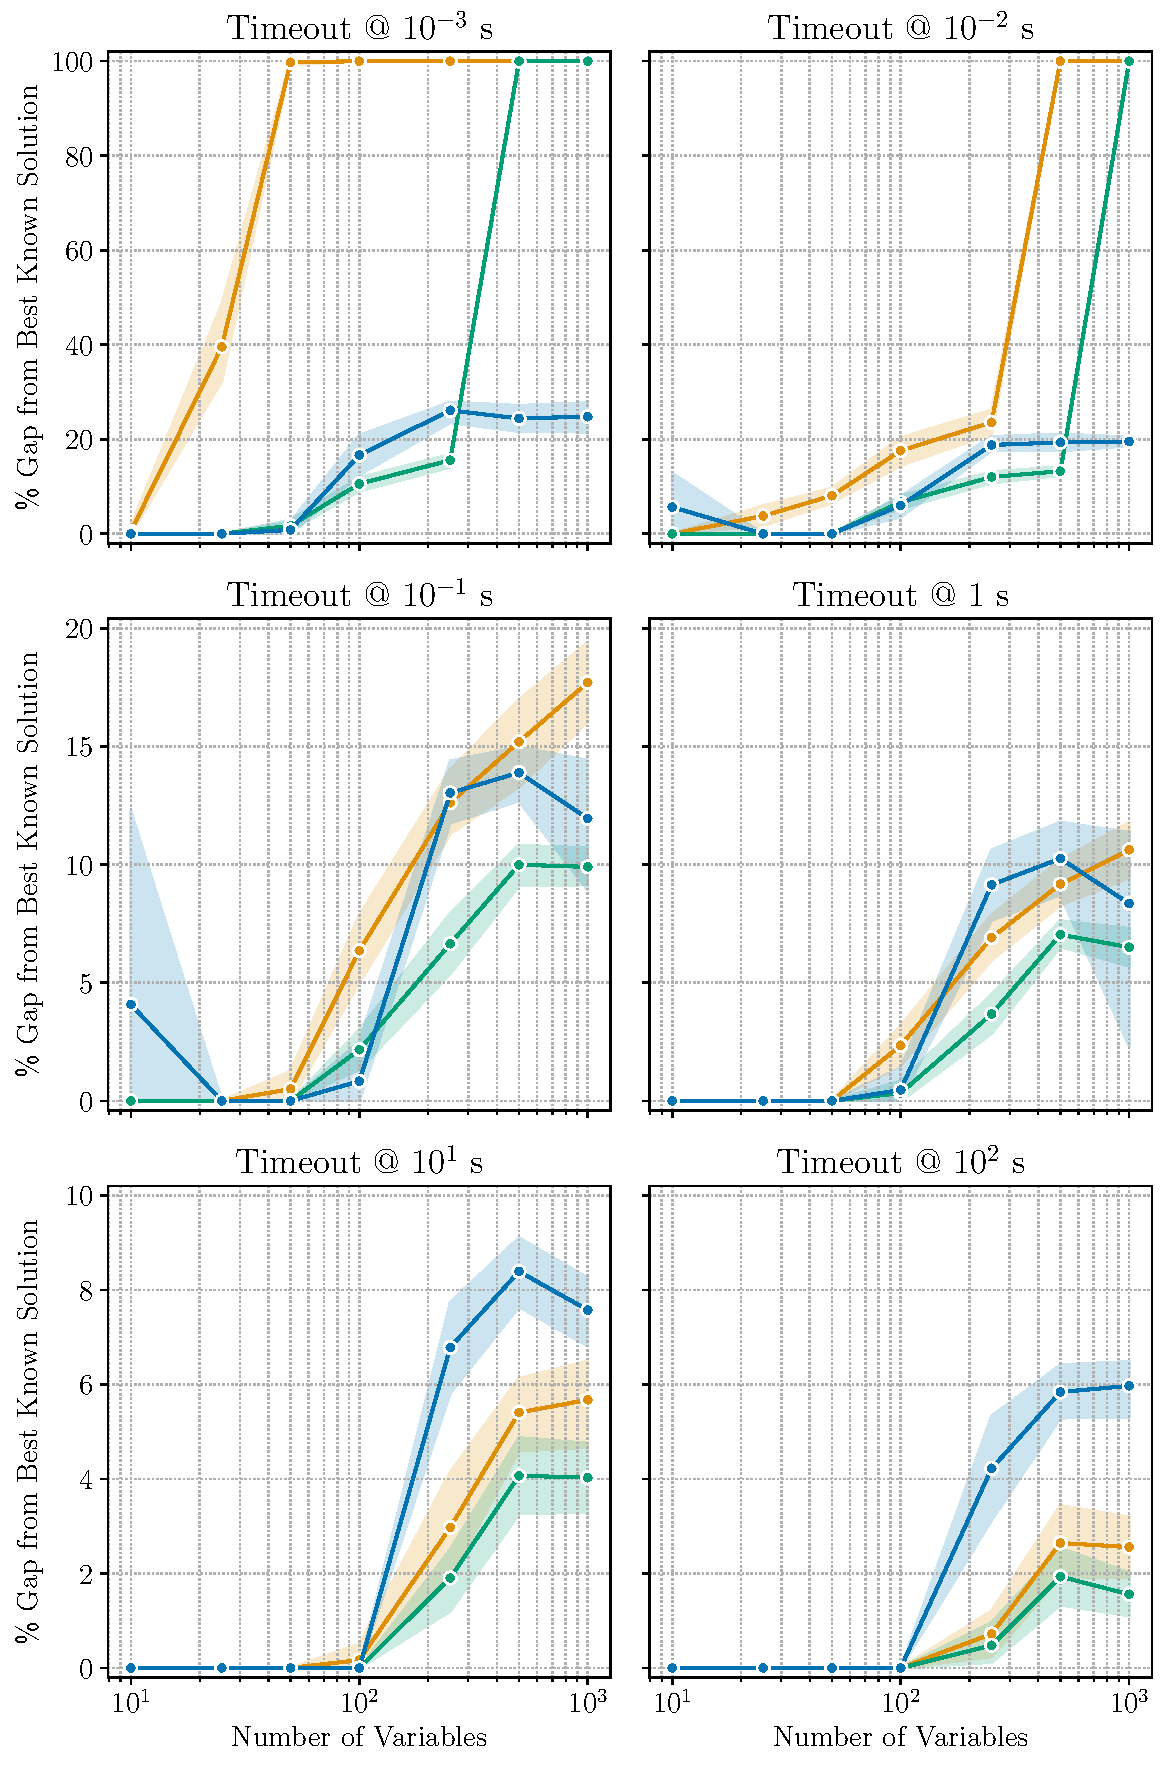
\includegraphics[width=\linewidth]{figures/mis_optimality_0.15.pdf}
    \vspace*{0.2cm}
    \end{subfigure}\\
    \begin{subfigure}{0.3\textwidth}
        
\includegraphics[width=\linewidth]{figures/legend.pdf}
    \end{subfigure}
    \caption{\secondrev{Percentage gap from the best known solution (BKS-Gap\%) for the QUBO workloads with QUBO matrices at $15\%$ density (lower is better). Results are shown for different timeouts of the QUBO solvers. Figure taken, with permission, from Pierro et al.~\cite{pierro2024solvingquboloihi2}.}}
    \label{fig:qubo_bksgap}
\end{figure}

\begin{figure}[t]
    \centering
        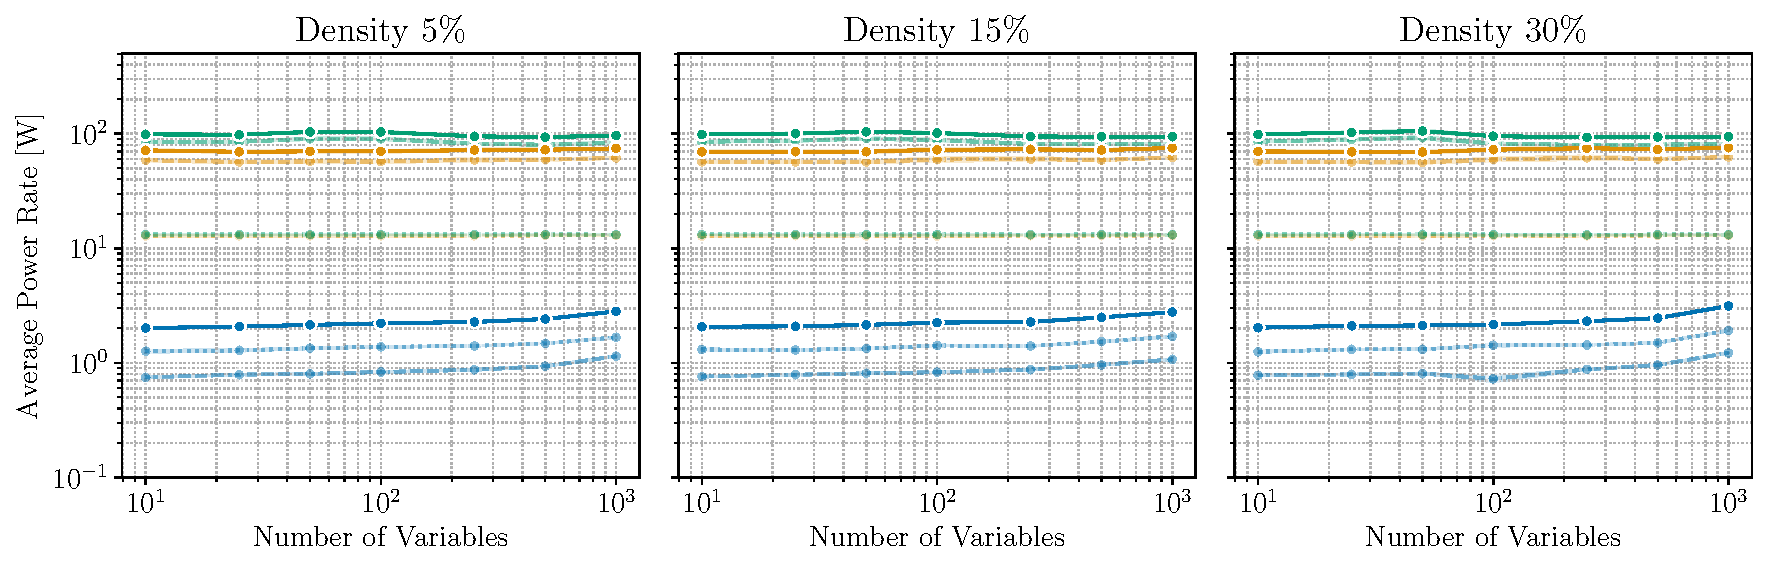
\includegraphics[width=\linewidth]{figures/mis_power.pdf}
    \vspace*{0.5cm}

\includegraphics[width=0.3\linewidth]{figures/legend.pdf}
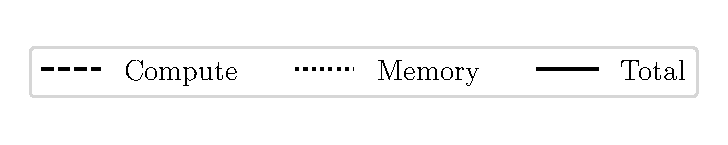
\includegraphics[width=0.35\linewidth]{figures/line_style_legend.pdf}
        \caption{\secondrev{Power consumption of the QUBO solvers running simulated annealing (SA) or TABU search on CPU, and the parallelized version of simulated annealing on Loihi 2. The CPU solvers require up to $37\times$ more power than the neuromorphic algorithm on Loihi 2. Since the QUBO workloads were run for a fixed timeout, differences in power consumption are equivalent to differences in energy consumption of the processors. Figure taken, with permission, from Pierro et al.~\cite{pierro2024solvingquboloihi2}.}}
        \label{fig:qubo_power}
\end{figure}

\secondrev{Three baselines are measured for the QUBO benchmark:
\begin{itemize}
    \item \textbf{Simulated Annealing (SA)} -- The simulated annealing solver uses Markov chain Monte Carlo (MCMC) sampling to probabilistically explore the search space. 
    \item \textbf{Tabu Search (TABU)} -- Tabu search solvers maintain and iterate a list of prohibited actions in order to prevent the search from remaining in local minima or revisiting states. Both the TABU and SA solver baselines use the D-Wave Samplers library~\cite{dwavesamplers} on an Intel Core i9-7920X desktop-class CPU, with power measured using Intel SoC Watch.
    \item \textbf{Loihi 2} -- The Loihi 2 neuromorphic system solver uses an SNN formulation of the simulated annealing algorithm which enables solving via neural dynamics, and parallelization via stochastic refractory periods. The baseline is implemented on one Loihi 2 chip on the 8-chip Kapoho Point board, and internal power instrumentation measures all compute and memory components of the chip.
\end{itemize}}

\secondrev{Figure~\ref{fig:qubo_bksgap} shows the optimality reached by the CPU- and Loihi 2-based solvers after different timeouts. For tight time constraints, at $10^{-2}$ seconds timeout or less, Loihi 2 finds feasible solutions to workloads $4\times$ larger than the CPU. But for timeout lasting $10$ seconds or longer, the CPU running TABU provides the lowest BKS-Gap, incentivizing algorithmic advances for neuromorphic optimization systems.}
\secondrev{Figure~\ref{fig:qubo_power} illustrates the power consumed during runtime. Across the workloads, the Loihi 2 solver requires $37.24\times$ less power compared to the best CPU solver.  
%All details on the solvers, benchmarking routine, and results have been provided by Pierro et al.~\cite{pierro2024solvingquboloihi2}.
}

\subsubsection*{Discussion and Future Work}
\secondrev{The initial baselines for the v1.0 system track compare correctness, timing, and efficiency of neuromorphic systems against conventional CPU systems in domains of both audio classification and optimization. Against mature, commercially-developed CPU systems, for both edge and server use cases, the neuromorphic systems show strong advantages in general efficiency, as well as further promises in terms of timing and correctness. 
%The benchmarks utilize collaboratively-defined task and methodology specifications, setting the groundwork for head-to-head neuromorphic system comparisons that will identify neuromorphic strengths and push towards standardization and development of better neuromorphic systems.
}

\secondrev{In future NeuroBench iterations, the system track benchmarks can be unified under common tooling, similar to the algorithm track. Software toolchains such as Lava~\cite{lava}, Fugu~\cite{aimone2019composing}, SPyNNaker~\cite{spynnaker}, and Samna~\cite{samna}, among others, have been developed to interface with specific hardware platforms. Many of the stacks are built with general paradigms to support extension to any backend, and the community is actively moving towards developing standards for deployment tools. The current v1.0 benchmark specifications allow for open algorithm and software design in order to demonstrate fully optimized performance for neuromorphic systems. As standards mature in the future, a core focus of the NeuroBench system track is to introduce a closed-algorithm benchmarking category that leverages the recently proposed NIR model description framework~\cite{NIR2024} as a general, cross-platform tool for benchmarking key workloads of interest across many different platforms.}